\chapter{Examples} \label{chap:examples}
The pruning algorithm is presented on several examples, where each of them has its purpose of being shown. The XOR problem (\cref{sec:example_xor}) should verify the ability of finding an optimal network structure. Section \ref{sec:example_ufi} comes with another 2D problem, where one feature carries more information than the other one. The Rule-plus-Exception problem in \cref{sec:example_rpe} deals with a minority of samples that has to be treated by a different net part than rule-based samples. The train problem (\cref{sec:example_trains}) is a working example of the feature selection procedure. The MNIST database (\cref{sec:example_mnist}) is widely used in machine learning and can be regarded as commonly known, hence it is an ideal example to present new methods on. Finally, in \cref{sec:example_speech} the pruning algorithm is analysed on a large dataset of phonemes.

\section{XOR Function} \label{sec:example_xor}
The standard Exclusive OR (XOR) function is defined by truth \cref{tab:examples:xor_function}. Based on this function one can build a classification problem of two features and two classes.

\begin{table}[H]
\centering
\begin{tabular}{|c|c||c|}
\hline
\textit{$ x_1 $} & \textit{$ x_2 $} & \textit{y} \\ \hline \hline
0                & 0                & 0          \\ \hline
0                & 1                & 1          \\ \hline
1                & 0                & 1          \\ \hline
1                & 1                & 0          \\ \hline
\end{tabular}
\caption{XOR function.}
\label{tab:examples:xor_function}
\end{table}

This problem serves perfectly for a demonstration of network optimization methods, as two optimal architectural solutions producing the XOR function are already known (\cref{fig:examples:xor_solutions}) \footnote{The known (e.g. from \citep{online:xor_solution}) minimal network architectures producing the XOR function $ [2, 2, 1] $ and $ [2, 3, 1] $ are adjusted to $ [2, 2, 2] $ and $ [2, 3, 2] $ in \cref{fig:examples:xor_solutions} in order to comply with the conventions introduced in \cref{chap:methods}. The number of output neurons always equals the number of classes. The number of hidden-output synapses might not be optimized in this study.}. 

\begin{figure}[H]
\centering
\begin{subfigure}{.4\textwidth}
  \centering
  \includegraphics[height=2cm]{xor_min1}
  \caption{Solution A.}
  \label{fig:examples:xor_min1}
\end{subfigure}
\begin{subfigure}{.4\textwidth}
  \centering
  \includegraphics[height=2cm]{xor_min2}
  \caption{Solution B.}
  \label{fig:examples:xor_min2}
\end{subfigure}
\caption{Optimal network architectures producing the XOR function.}
\label{fig:examples:xor_solutions}
\end{figure}

With this knowledge we can prove that the pruning algorithm is (or is not) able to find the optimal solution. If the method is correct, it should end up with one of the shown architectures (\cref{fig:examples:xor_min1} or \cref{fig:examples:xor_min2}).

The truth \cref{tab:examples:xor_function} ruled the generation of a 2D dataset illustrated in \cref{fig:examples:dataset_xor}. The two classes can be linearly separated by two lines (corresponding to two neurons, see \cref{fig:examples:xor_min1}) and each class consists of 1000 samples. Each sample was randomly assigned to one of the two possible points belonging to its class (e.g. (0,0) or (1,1) for class 0) and then randomly placed in the surounding area within a specified range ($ r = \frac{\sqrt{2}}{4} $).

The samples of each class were then splitted into three sets in the following manner: $ 80\% $ to a training set, $ 10\% $ to a validation set and $ 10\% $ to a testing set.

\begin{figure}[H]
\centering
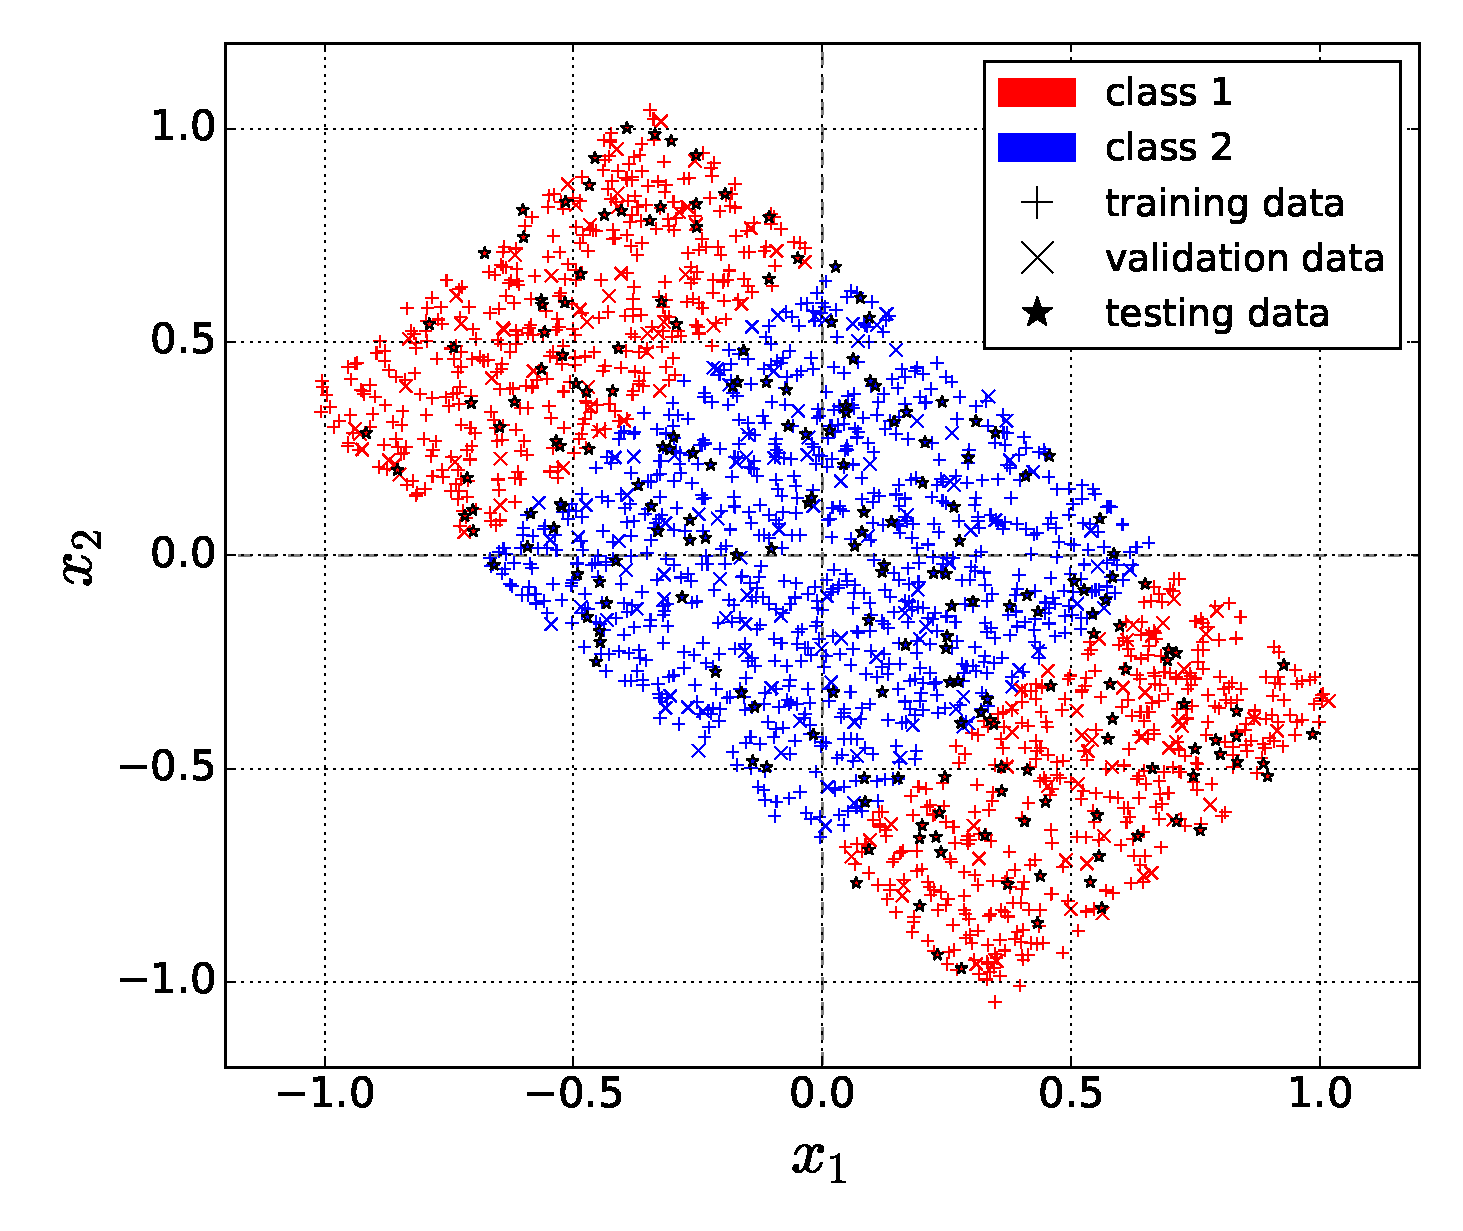
\includegraphics[width=0.9\textwidth]{dataset_xor.eps}
\caption{The XOR dataset.}
\label{fig:examples:dataset_xor}
\end{figure}

The goal of this example is to show that the pruning algorithm finds one of the known minimal network structures (\cref{fig:examples:xor_solutions}). An oversized network $ [2, 50, 2] $ is used as the starting point. The following \cref{tab:examples:xor_settings} shows all the experiment settings.

\begin{table}[H]
\centering
\scalebox{0.95}{
\begin{tabular}{|l|c|l|c|l|c|}
\hline
\multicolumn{2}{|c|}{\textit{initial network}} & \multicolumn{2}{c|}{\textit{learning parameters}} & \multicolumn{2}{c|}{\textit{pruning parameters}} \\ \hline
structure             & {[}2, 50, 2{]}         & learning rate                  & 0.3              & required accuracy             & 1.0              \\ \hline
n synapses            & 200                    & number of epochs               & 50               & retrain                       & True             \\ \hline
transfer fcn          & sigmoid                & minibatch size                 & 1                & retraining epochs             & 50               \\ \hline
\end{tabular}}
\caption{Experiment settings for the XOR example.}
\label{tab:examples:xor_settings}
\end{table}

\subsection*{Results: XOR Function}
\cref{fig:examples:pruning_process_xor} describes the pruning process. We can see the number of synapses, the network structure and the classification accuracy for single pruning steps (see [PA]). When the required accuracy ($ 1.0 $) was not reached, the corresponding steps are transparent in the figure, indicating they were forgotten.

\begin{figure}[H]
\centering
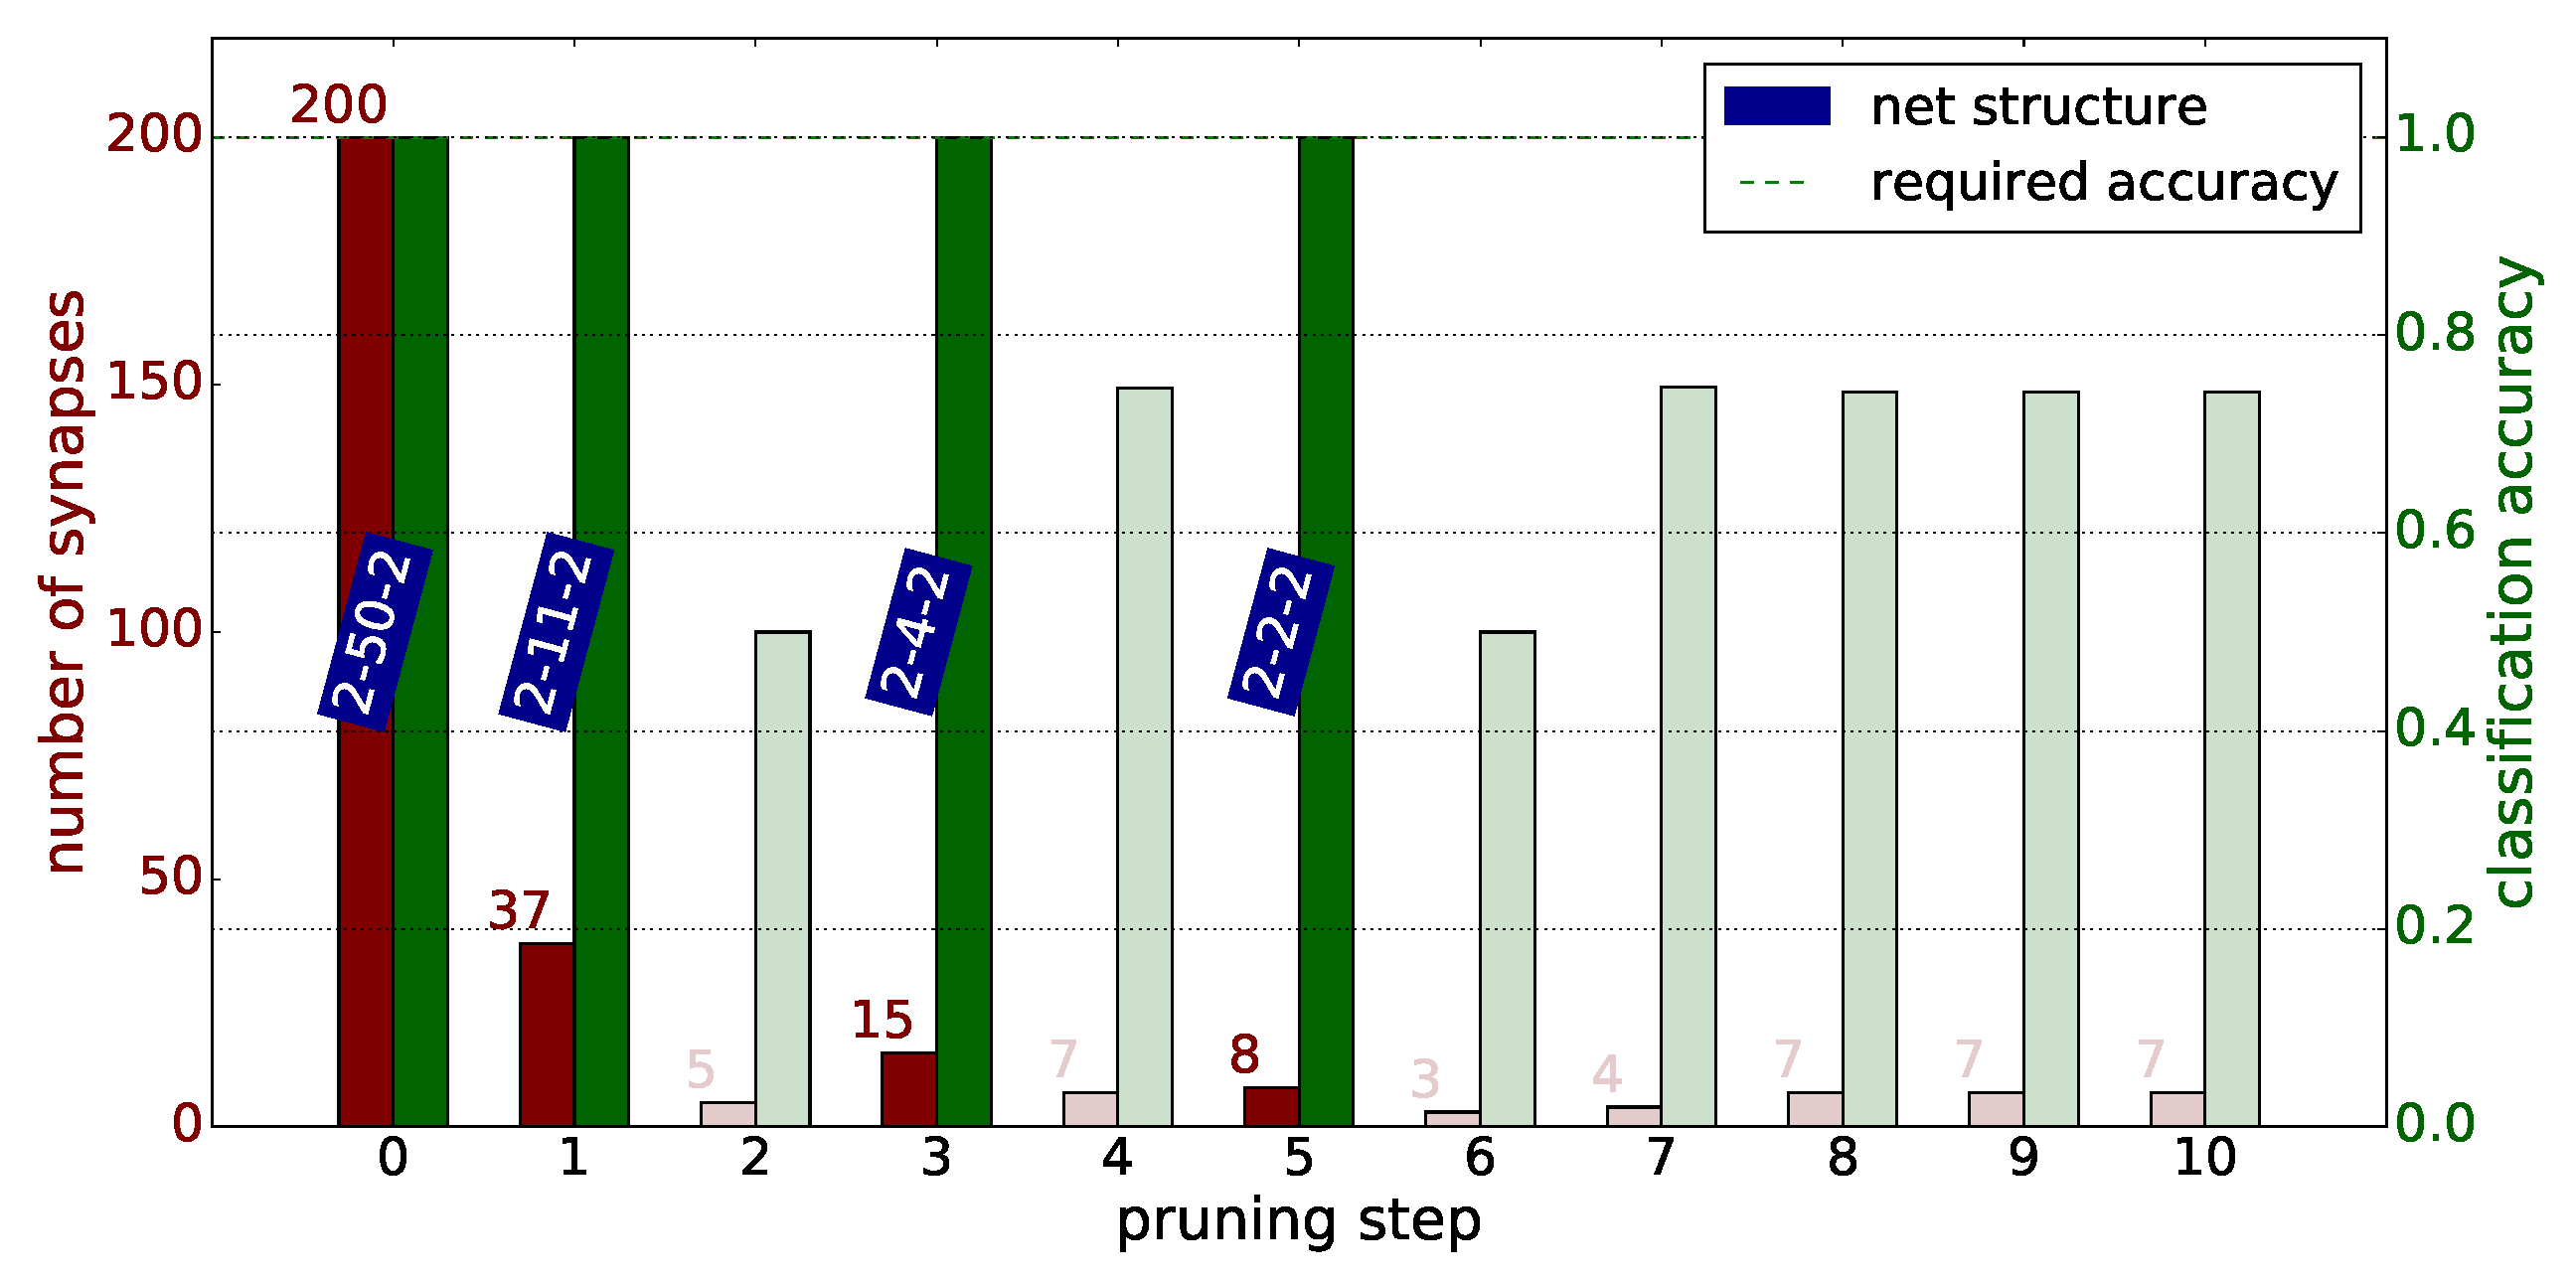
\includegraphics[width=\textwidth]{pruning_process_xor.eps}
\caption{Illustration of the pruning procedure applied on XOR dataset (selected observation).}
\label{fig:examples:pruning_process_xor}
\end{figure}

In \cref{fig:examples:pruning_result_xor} the hypothesis of this experiment is confirmed. We ran $ 100 $ observations of the experiment. In \cref{fig:examples:pie_xor} we can see that in $ 47 $ out of $ 100 $ cases the pruning algorithm changed the network to $ [2, 2, 2] $ architecture (\cref{fig:examples:xor_min1}), in $ 45\% $ of the cases it resulted with $ [2, 3, 2] $ (\cref{fig:examples:xor_min2}) and only in $ 8\% $ it failed to find the optimal architecture. \cref{fig:examples:result_synapses_xor} gives statistics for the final number of synapses in these three cases.

\begin{figure}[H]
\centering
\begin{subfigure}{.4\textwidth}
  \centering
  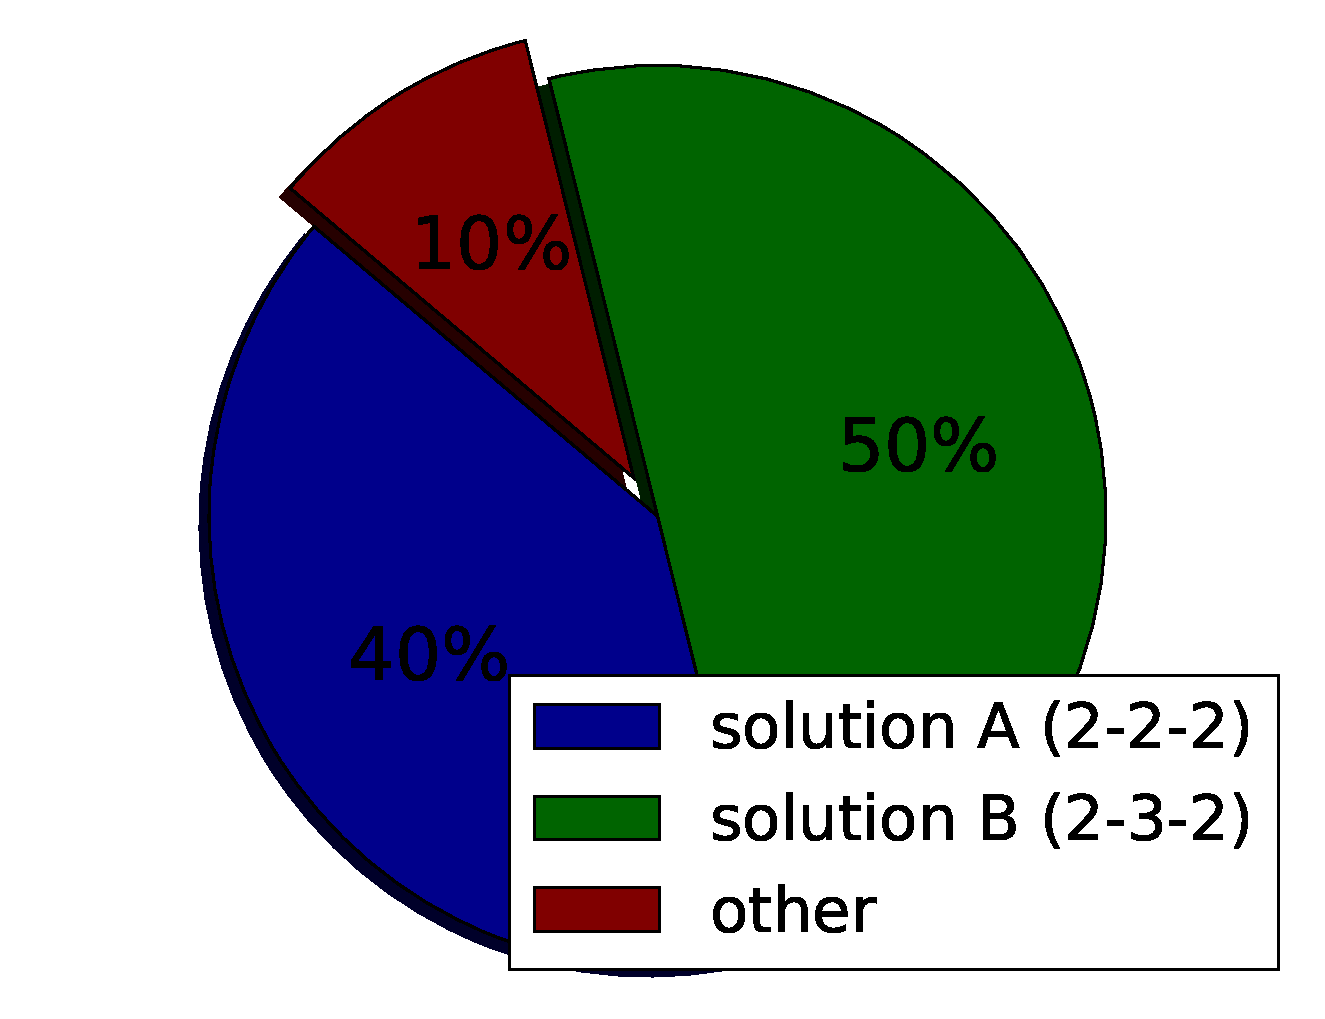
\includegraphics[height=4cm]{pruning_result_pie_xor.eps}
  \caption{Network structure after pruning (100 observations).}
  \label{fig:examples:pie_xor}
\end{subfigure}
\begin{subfigure}{.4\textwidth}
  \centering
  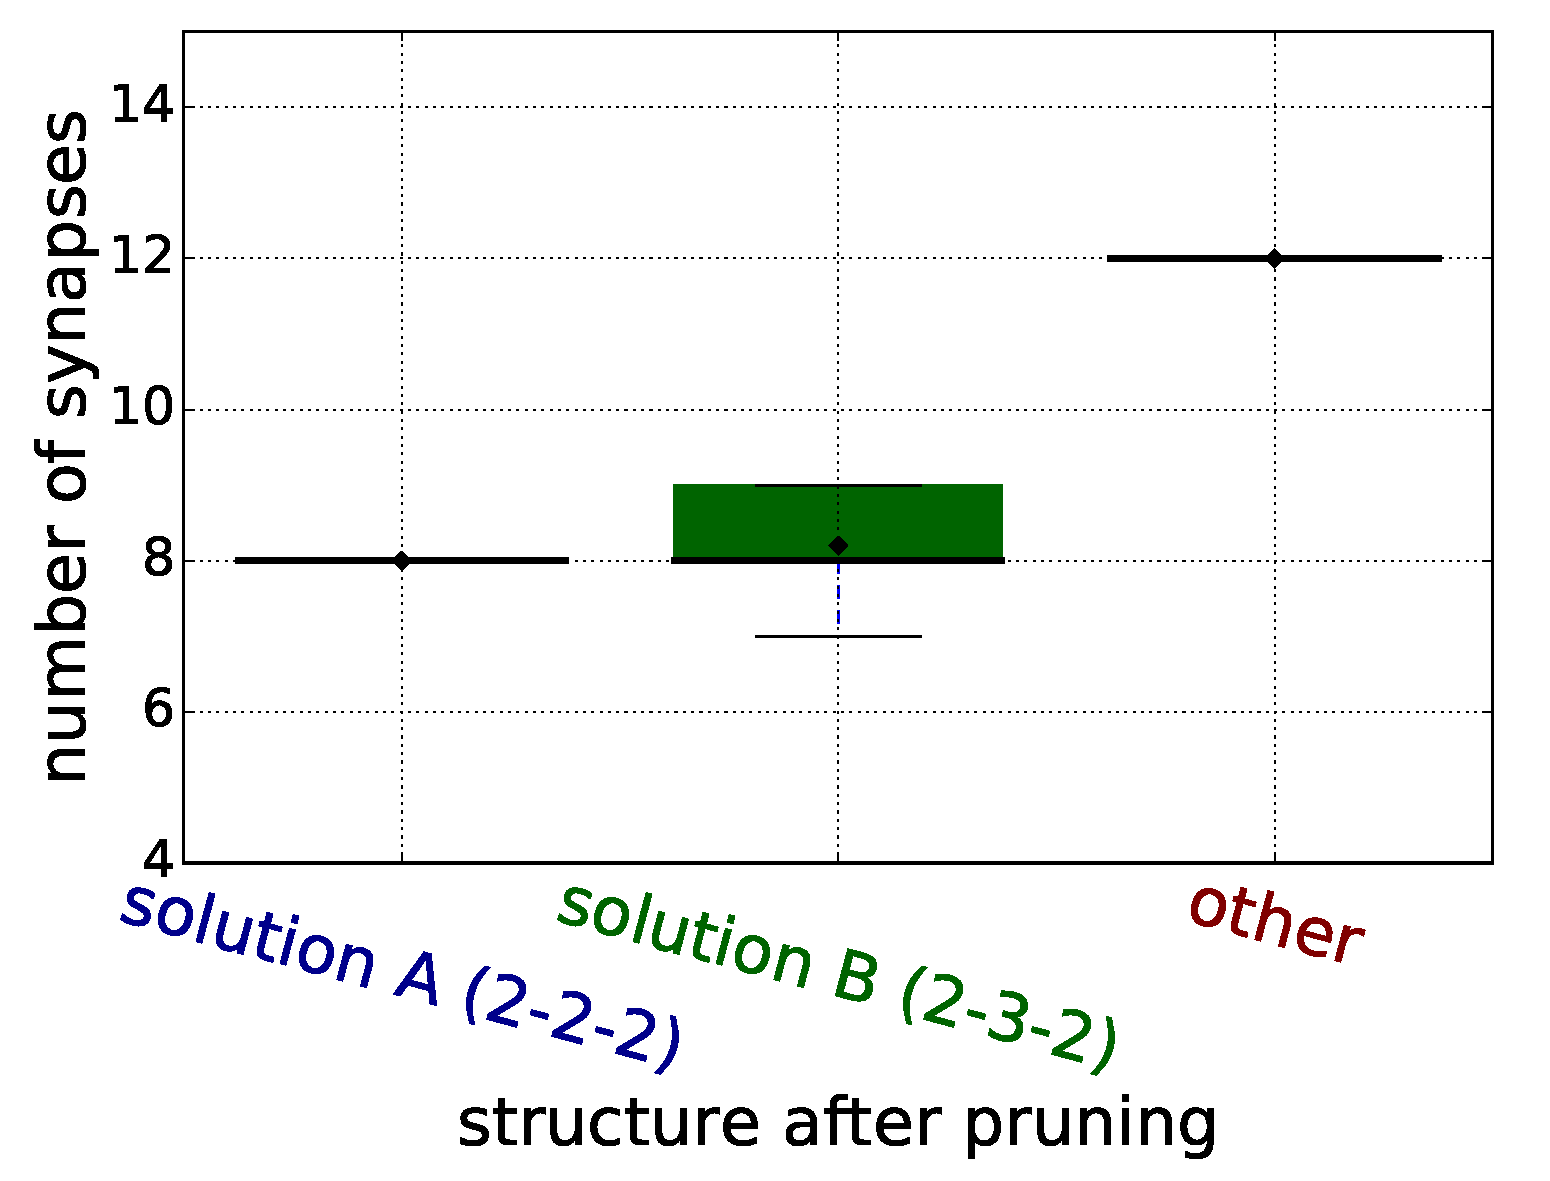
\includegraphics[height=4cm]{pruning_result_synapses_xor.eps}
  \caption{Number of synapses after pruning (100 observations).}
  \label{fig:examples:result_synapses_xor}
\end{subfigure}
\caption{Pruning results for XOR dataset.}
\label{fig:examples:pruning_result_xor}
\end{figure}

\section{Unbalanced Feature Information} \label{sec:example_ufi}
This example is adopted from \citep{karnin}. The problem is again two-dimensional having two non-overlapping classes as depicted in \cref{fig:examples:dataset_unbfea}. The samples are uniformly distributed in $ [-1, 1] $ x $ [-1, 1] $ and the classes are equally probable, separated by two lines in 2D space ($ x_1 = a $ and $ x_2 = b $, where $ a = 0.1 $ and $ b = \frac{2}{a+1} - 1 \approx 0.82 $). Clearly, the problem can be solved by two neurons, similarly as the previous one.

What is interesting about this two-classes layout is that feature $ x_1 $ is much more important for the global classification accuracy than feature $ x_2 $. Having $ x_1 $ information, based on \cref{fig:examples:dataset_unbfea} one could potentially classify more than $ 90\% $ of the samples. Opposite of that, we cannot say much with information from feature $ x_2 $ only. And this is something that also the pruning algorithm should find out.

\begin{figure}[H]
\centering
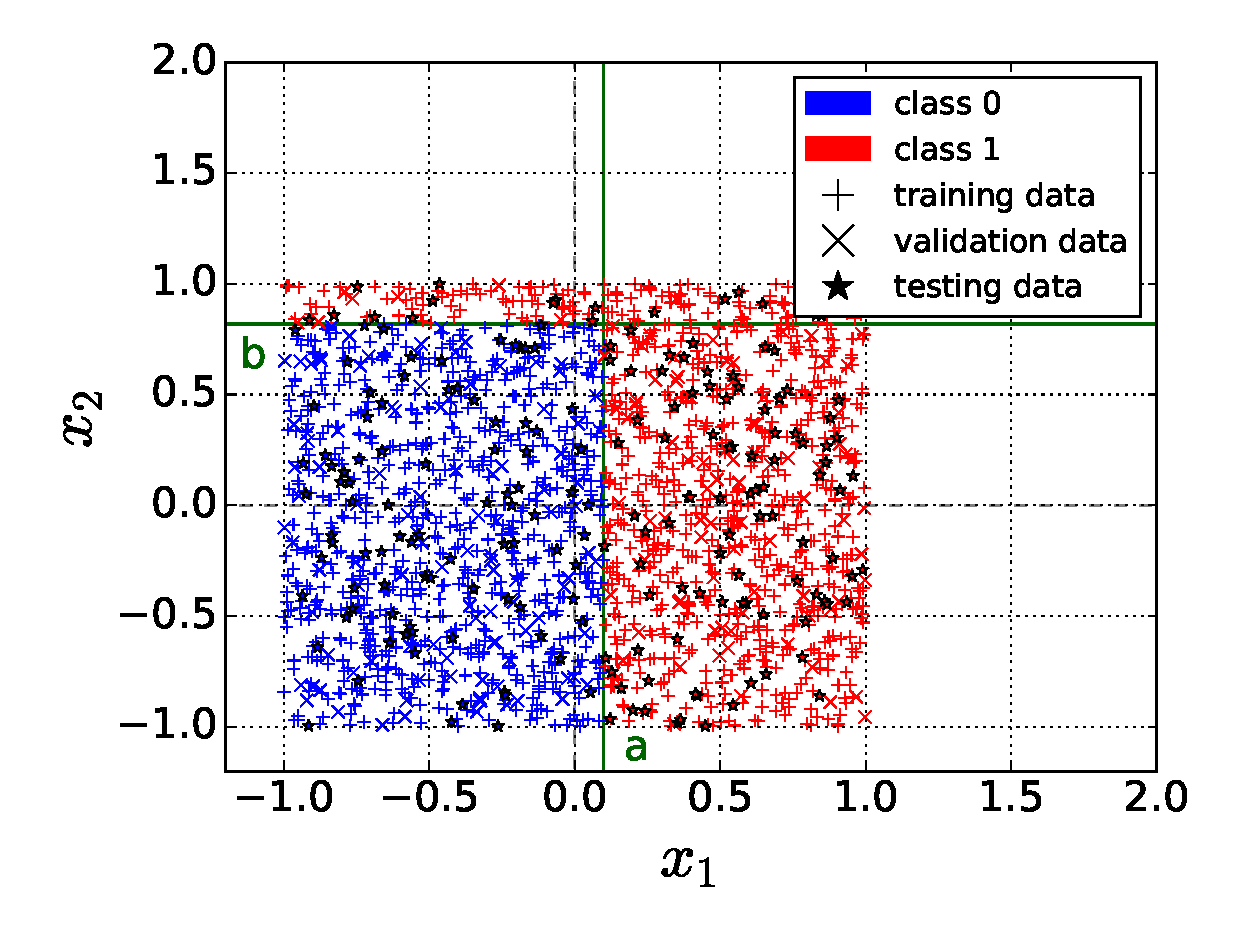
\includegraphics[width=0.8\textwidth]{dataset_unbfea.eps}
\caption{The UFI dataset.}
\label{fig:examples:dataset_unbfea}
\end{figure}

Hence, we focus on synapses connecting the input and the hidden layer (shortly input-hidden synapses). We know the required network structure is $ [2, 2, 2] $, as two lines are needed to separate the data in 2D space. Actually, we even know the lines must be parallel to coordinate axes, which means that each of the hidden units needs one of the features only. Therefore, the first hypothesis here is that pruning of input-hidden synapses should result in one of the cases in \cref{fig:examples:unbfea_hypos}.

\begin{figure}[H]
\centering
\begin{subfigure}{.4\textwidth}
  \centering
  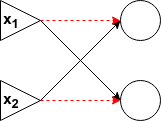
\includegraphics[height=2cm]{unbfea_hypo1}
  \caption{Pruning result 1.}
  \label{fig:examples:unbfea_hypo1}
\end{subfigure}
\begin{subfigure}{.4\textwidth}
  \centering
  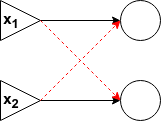
\includegraphics[height=2cm]{unbfea_hypo2}
  \caption{Pruning result 2.}
  \label{fig:examples:unbfea_hypo2}
\end{subfigure}
\caption{Expected pruning of input-hidden synapses (UFI problem).}
\label{fig:examples:unbfea_hypos}
\end{figure}

To prove this behaviour, we ran an experiment with settings in \cref{tab:examples:unbfea_settings}.

\begin{table}[H]
\centering
\scalebox{0.95}{
\begin{tabular}{|l|c|l|c|l|c|}
\hline
\multicolumn{2}{|c|}{\textit{initial network}} & \multicolumn{2}{c|}{\textit{learning parameters}} & \multicolumn{2}{c|}{\textit{pruning parameters}} \\ \hline
structure             & {[}2, 2, 2{]}          & learning rate                  & 0.7              & required accuracy             & 0.98             \\ \hline
n synapses            & 8                      & number of epochs               & 50               & retrain                       & True             \\ \hline
transfer fcn          & sigmoid                & minibatch size                 & 1                & retraining epochs             & 50               \\ \hline
\end{tabular}}
\caption{Experiment settings for the UFI example.}
\label{tab:examples:unbfea_settings}
\end{table}

The second hypothesis is that the synapse connected to the first feature ($ x_1 $) is more important and therefore, the other synapse (the one connected to feature $ x_2 $) should always be removed first.

\subsection*{Results: Unbalanced Feature Information}
In \cref{fig:examples:pruning_result_pie_unbfea} the first hypothesis is confirmed. We ran the experiment $ 100 $ times. In $ 48 $ cases, the pruning of input-hidden synapses finished with the result shown in \cref{fig:examples:unbfea_hypo1} and it finished with the result shown in \cref{fig:examples:unbfea_hypo2} in $ 44\% $ of the cases.

\begin{figure}[H]
\centering
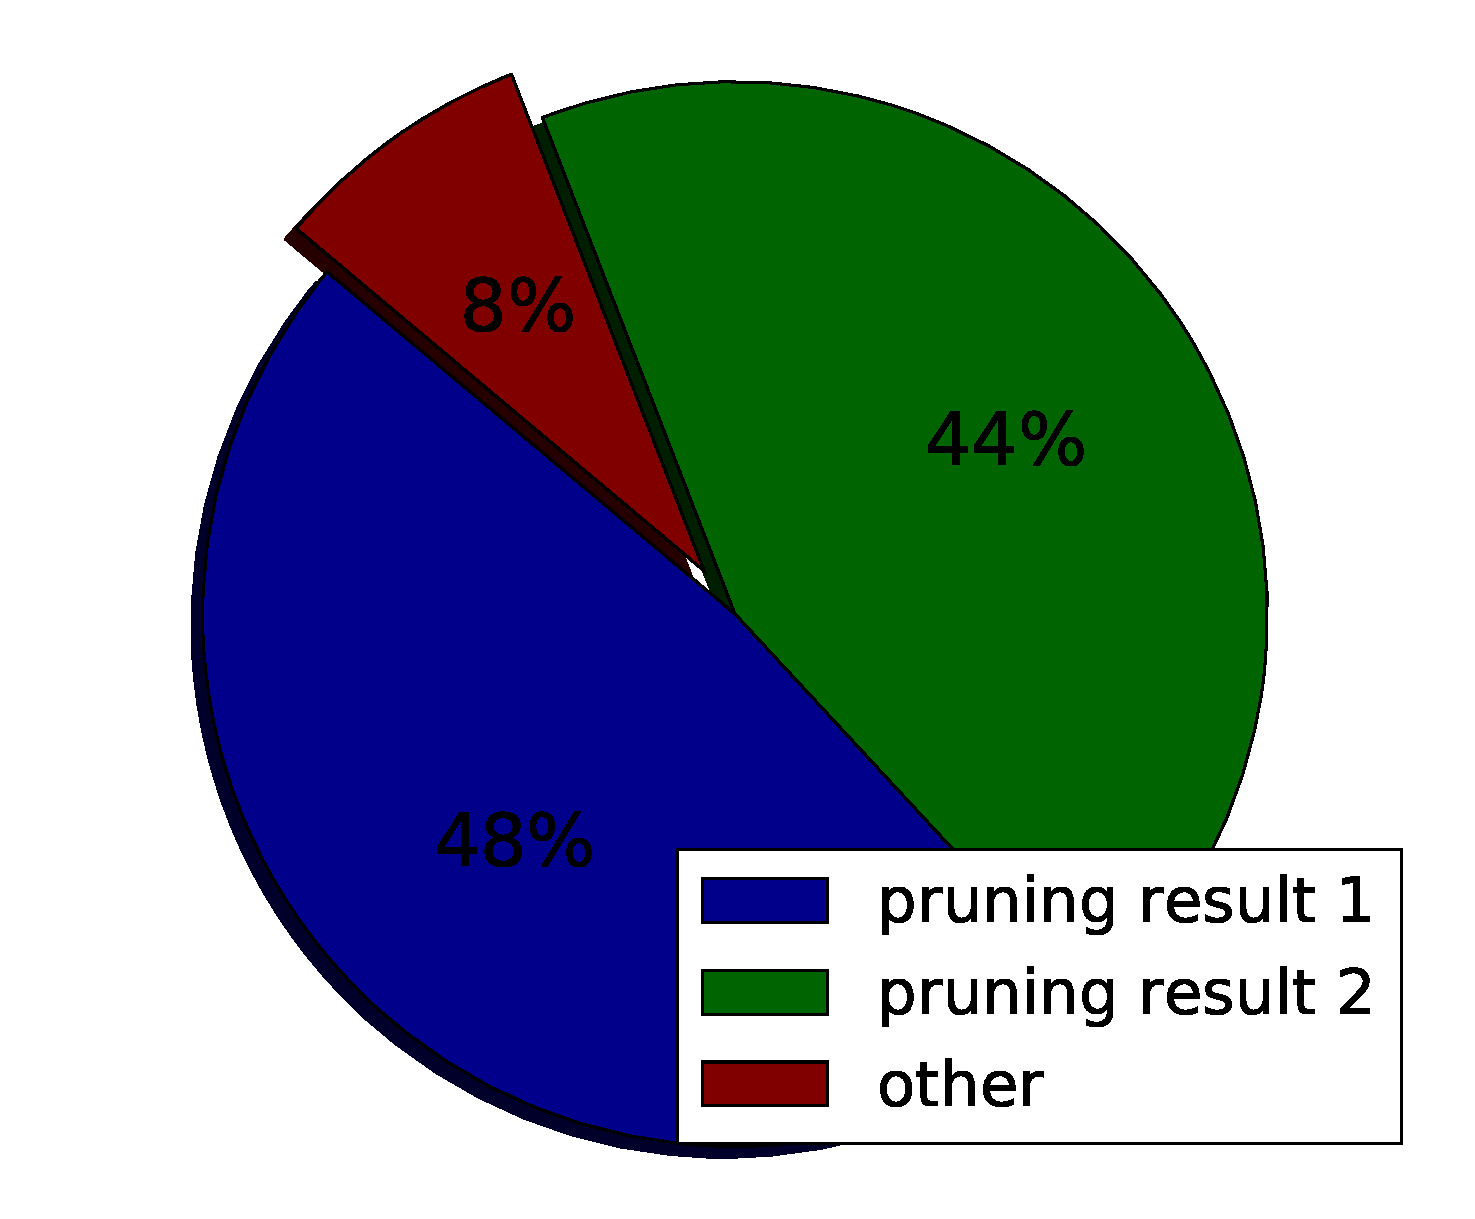
\includegraphics[width=0.5\textwidth]{pruning_result_pie_unbfea.eps}
\caption{Results of pruning (see \cref{fig:examples:unbfea_hypos}) input-hidden synapses (100 observations, UFI example).}
\label{fig:examples:pruning_result_pie_unbfea}
\end{figure}

In other words, with a probability of $ 92\% $ the algorithm is able to find the axis-parallel lines and reveals that each of the lines needs the information from corresponding feature only. In the remaining $ 8\% $ of the cases the pruning resulted with more than two input-hidden synapses.

The second hypothesis is confirmed in \cref{fig:examples:unbfea_synapse_weight_change}. The synapses's significance factor was always (100 observations) greater for the synapse coming from feature $ x_1 $ than for the synapse connected to $ x_2 $. By definition (see [PA]), the pruning method eliminates the synapses with low significance factors first, therefore the information coming from feature $ x_1 $ would live longer in the network than the $ x_2 $ information.

Let's try to explain this result. Consider $ w_{r1} $ to be the weight of the synapse connecting the $ x_1 $ feature and $ r^{th} $ hidden neuron (with bias $ b_r$) and $ w_{s2} $ to be the weight of the synapse coming from feature $ x_2 $ to $ s^{th} $ hidden neuron (with bias $ b_s $), then by neuron definition \citep{article:perceptron} we created two lines, perpendicular one to each other, as follows.
\begin{align}
w_{r1} \cdot x_1 + 0 \cdot x_2 + b_r &= 0 \\
x_1 &= -\frac{b_r}{w_{r1}} \\
0 \cdot x_1 + w_{s2} \cdot x_2 + b_s &= 0 \\
x_2 &= -\frac{b_s}{w_{s2}}
\end{align}
In \cref{fig:examples:dataset_unbfea} we see that $ a < b $. To generalize the problem (assuming normalised feature vectors, see \cref{chap:methods}) we state $ |a| < |b| $, meaning we want:
\begin{align}
|-\frac{b_r}{w_{r1}}| &< |-\frac{b_s}{w_{s2}}|
\end{align}
Hence we expect:
\begin{align}
|w_{r1}| &> |w_{s2}|
\end{align}

Out of this we expect a weight magnitude to be greater for more important synapses.

\begin{figure}[H]
\centering
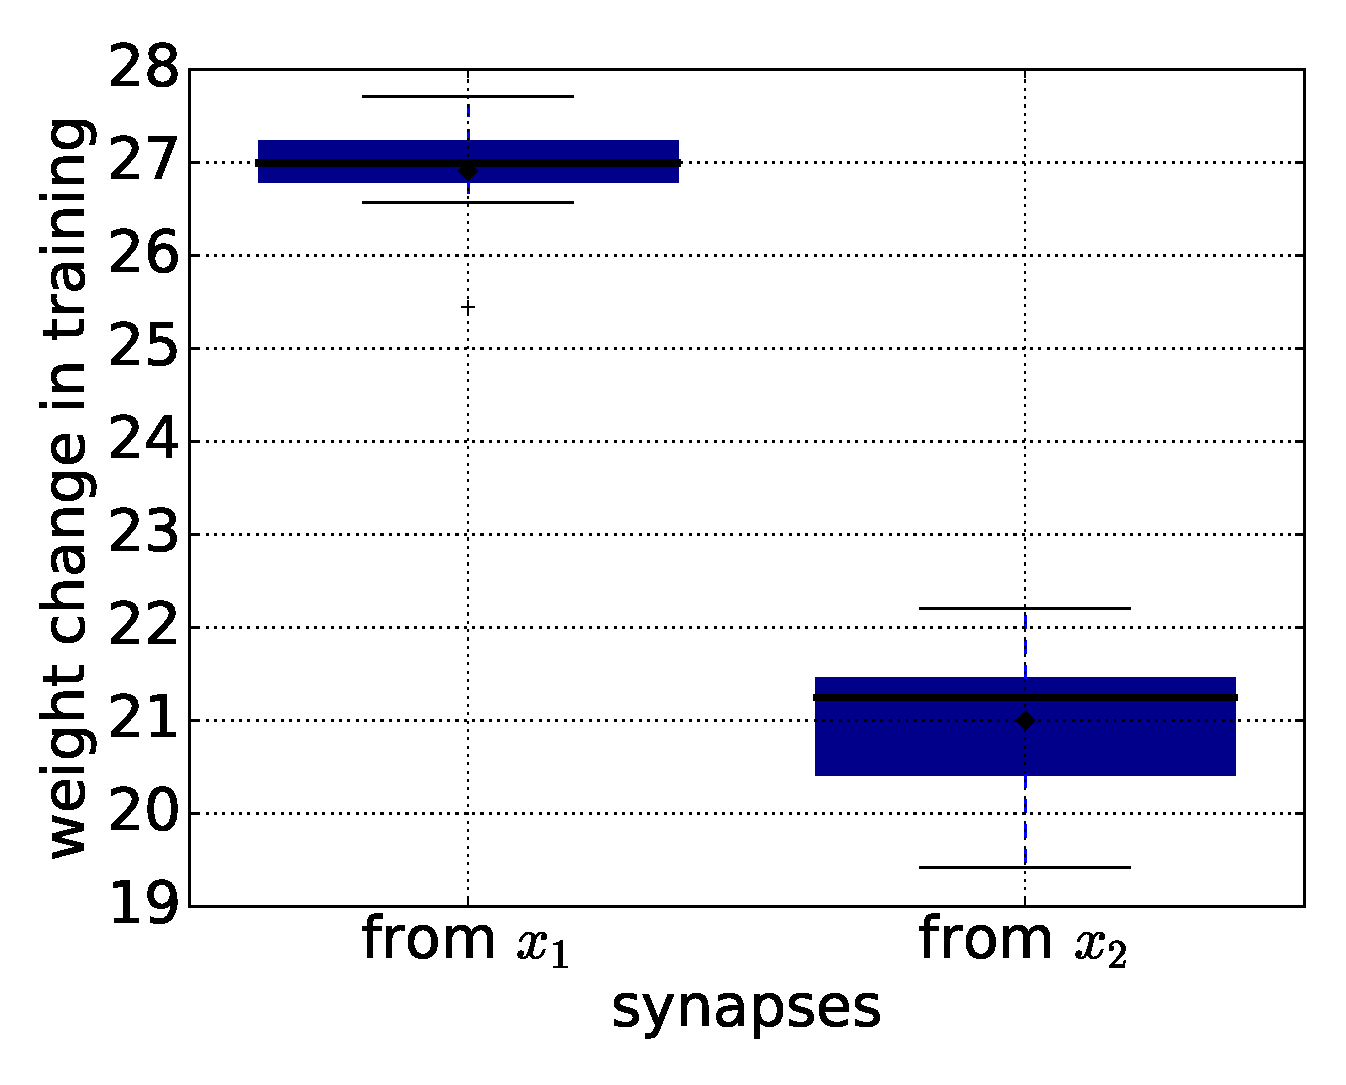
\includegraphics[width=0.5\textwidth]{unbfea_synapse_weight_change.eps}
\caption{Weight change in training for the remaining input-hidden synapses (100 observations).}
\label{fig:examples:unbfea_synapse_weight_change}
\end{figure}

The weight magnitude seems to be a perfect measure to find feature significance factor. However, as we do not use a weight decay (see the learning approach in \cref{chap:methods}), in general the more epochs we learn the greater weight magnitudes we get. Therefore small initial weight values do not affect the result significantly and so we can state:

\begin{equation}
|w_{ji}(t)| \approx |w_{ji}(t) - w_{ji}(0)|
\end{equation}

where $ w_{ji}(0) \in N(0,1) $ is the initial value of weight $ w_{ji} $ and $ t $ is time. Summing it up we can say that the \texttt{kitt} measure [ref] based on weight change is equally good as the magnitude measure assuming enough training epochs (e.g. 50).

\section{Rule-plus-Exception} \label{sec:example_rpe}
This four-dimensional problem is originally adopted from \citep{mozer_smolensky} and is also used in \citep{karnin}. The task is to learn another Boolean function: $ AB+\overline{A} \, \overline{B} \, \overline{C} \, \overline{D} $. A single function output should be on (i.e. equals 1) when both $ A $ and $ B $ are on, which is the \textit{rule}, and it should also be on when the \textit{exception} $ \overline{A} \, \overline{B} \, \overline{C} \, \overline{D} $ occurs.

Clearly, the \textit{rule} occurs more often than the \textit{exception}, therefore the samples corresponding with the \textit{rule} should be more important for the global classification accuracy. The hypothesis is that the pruning method should suggest the part of network, which deals with the \textit{exception}, to be eliminated first - before network elements dealing with the \textit{rule}.

To test this hypothesis, a dataset of $ 10000 $ samples was generated. Each sample consists of four features: $ [a, b, c, d] $. Each of these features (for every sample) was randomly set to be \textit{on} ($ 1 $) or \textit{off} ($ 0 $). Then, whenever the \textit{rule} occured ($ a = 1 \wedge b = 1 $), the sample was assigned to class $ 1 $ (as a \textit{rule} sample). If the \textit{exception} occured ($ a = 0 \wedge b = 0 \wedge c = 0 \wedge d = 0 $), the sample was also labeled as $ 1 $ (as an \textit{exception} sample). Otherwise, the sample was assigned to class $ 0 $. Thereby the generated dataset consisted of:

\begin{itemize}
\item $ 2511 $ \textit{rule} samples (class $ 1 $);
\item $ 649 $ \textit{exception} samples (class $ 1 $);
\item $ 6840 $ samples in class $ 0 $.
\end{itemize}

The function is expected to be learned by two hidden neurons, one dealing with the \textit{rule} and the other one with the \textit{exception}. We focus on input-hidden synapses again. Two possible expected pruning results are shown in \cref{fig:examples:rpe_hypos}.

\begin{figure}[H]
\centering
\begin{subfigure}{.4\textwidth}
  \centering
  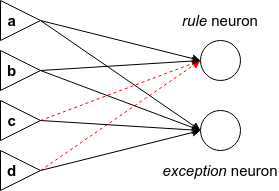
\includegraphics[height=3.5cm]{rpe_hypo1}
  \caption{Pruning result 1.}
  \label{fig:examples:rpe_hypo1}
\end{subfigure}
\begin{subfigure}{.4\textwidth}
  \centering
  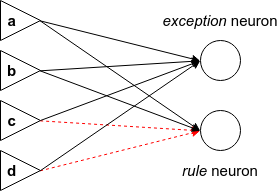
\includegraphics[height=3.5cm]{rpe_hypo2}
  \caption{Pruning result 2.}
  \label{fig:examples:rpe_hypo2}
\end{subfigure}
\caption{Expected pruning of input-hidden synapses (RPE problem).}
\label{fig:examples:rpe_hypos}
\end{figure}

We ran the learning-pruning procedure with the settings listed in \cref{tab:examples:rpe_settings}.

\begin{table}[H]
\centering
\scalebox{0.95}{
\begin{tabular}{|l|c|l|c|l|c|}
\hline
\multicolumn{2}{|c|}{\textit{initial network}} & \multicolumn{2}{c|}{\textit{learning parameters}} & \multicolumn{2}{c|}{\textit{pruning parameters}} \\ \hline
structure             & {[}2, 2, 2{]}          & learning rate                  & 1.0              & required accuracy             & 1.0             \\ \hline
n synapses            & 8                      & number of epochs               & 50               & retrain                       & True             \\ \hline
transfer fcn          & sigmoid                & minibatch size                 & 1                & retraining epochs             & 50               \\ \hline
\end{tabular}}
\caption{Experiment settings for the RPE example.}
\label{tab:examples:rpe_settings}
\end{table}

\subsection*{Results: Rule-plus-Exception}
\cref{fig:examples:pruning_result_pie_rpe} supports the hypothesis that one hidden neuron forms the \textit{rule} and the other one the \textit{exception}. With a probability of $ 97\% $ the pruning finished with one of the structures in \cref{fig:examples:rpe_hypos}.

\begin{figure}[H]
\centering
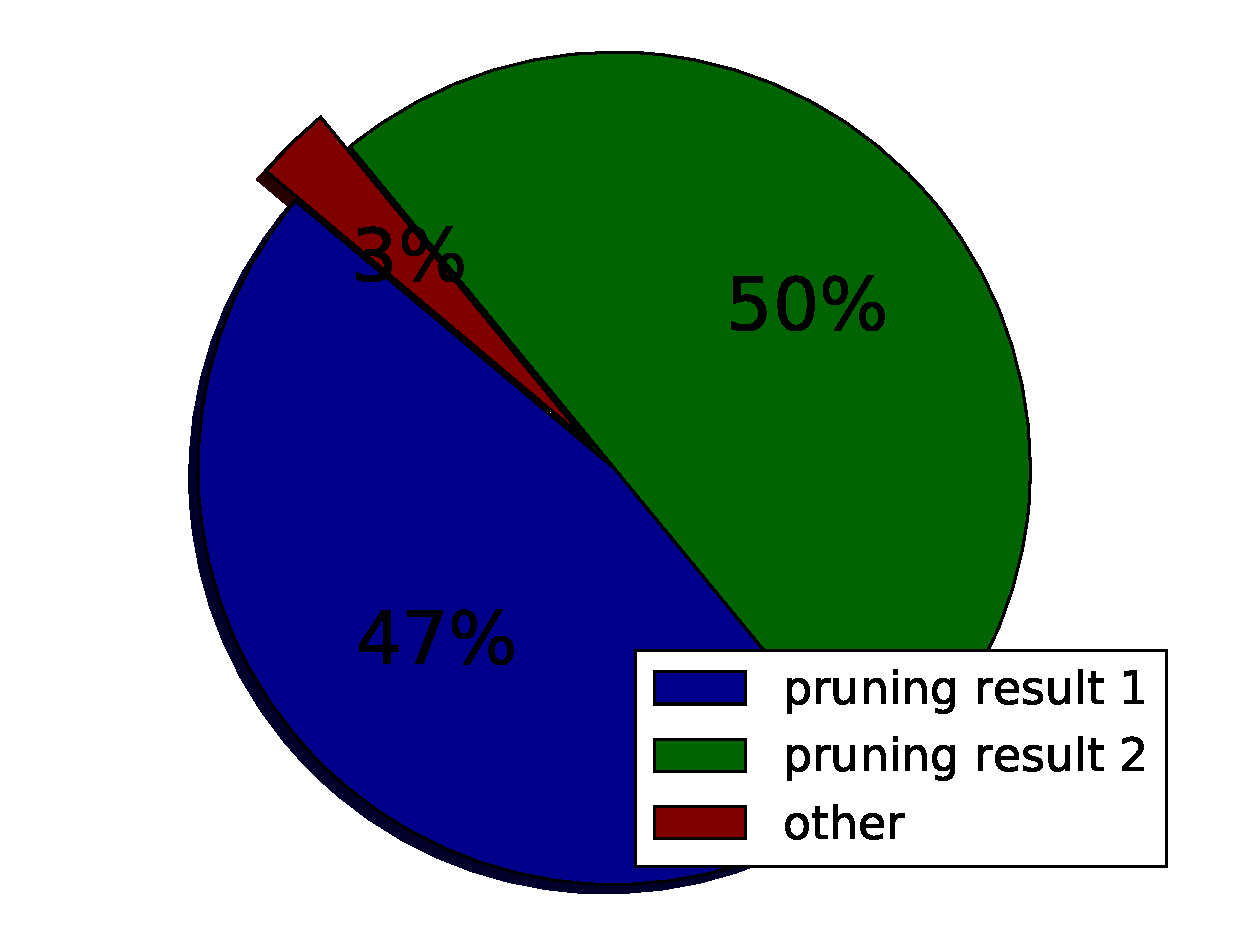
\includegraphics[width=0.5\textwidth]{pruning_result_pie_rpe.eps}
\caption{Results of pruning (see \cref{fig:examples:rpe_hypos}) input-hidden synapses (100 observations, RPE example).}
\label{fig:examples:pruning_result_pie_rpe}
\end{figure}

The same thing is confirmed by \cref{fig:examples:pruning_result_rpe}. It shows weight change in training (\texttt{kitt} significance factor) for all 8 input-hidden synapses. We can see that synapses connecting the \textit{rule} neuron with feature \textit{c} ($ s_{rc}) $ and feature \textit{d} ($ s_{rd} $) were suggested as least important (resulted in structures in \cref{fig:examples:rpe_hypos}).

\begin{figure}[H]
\centering
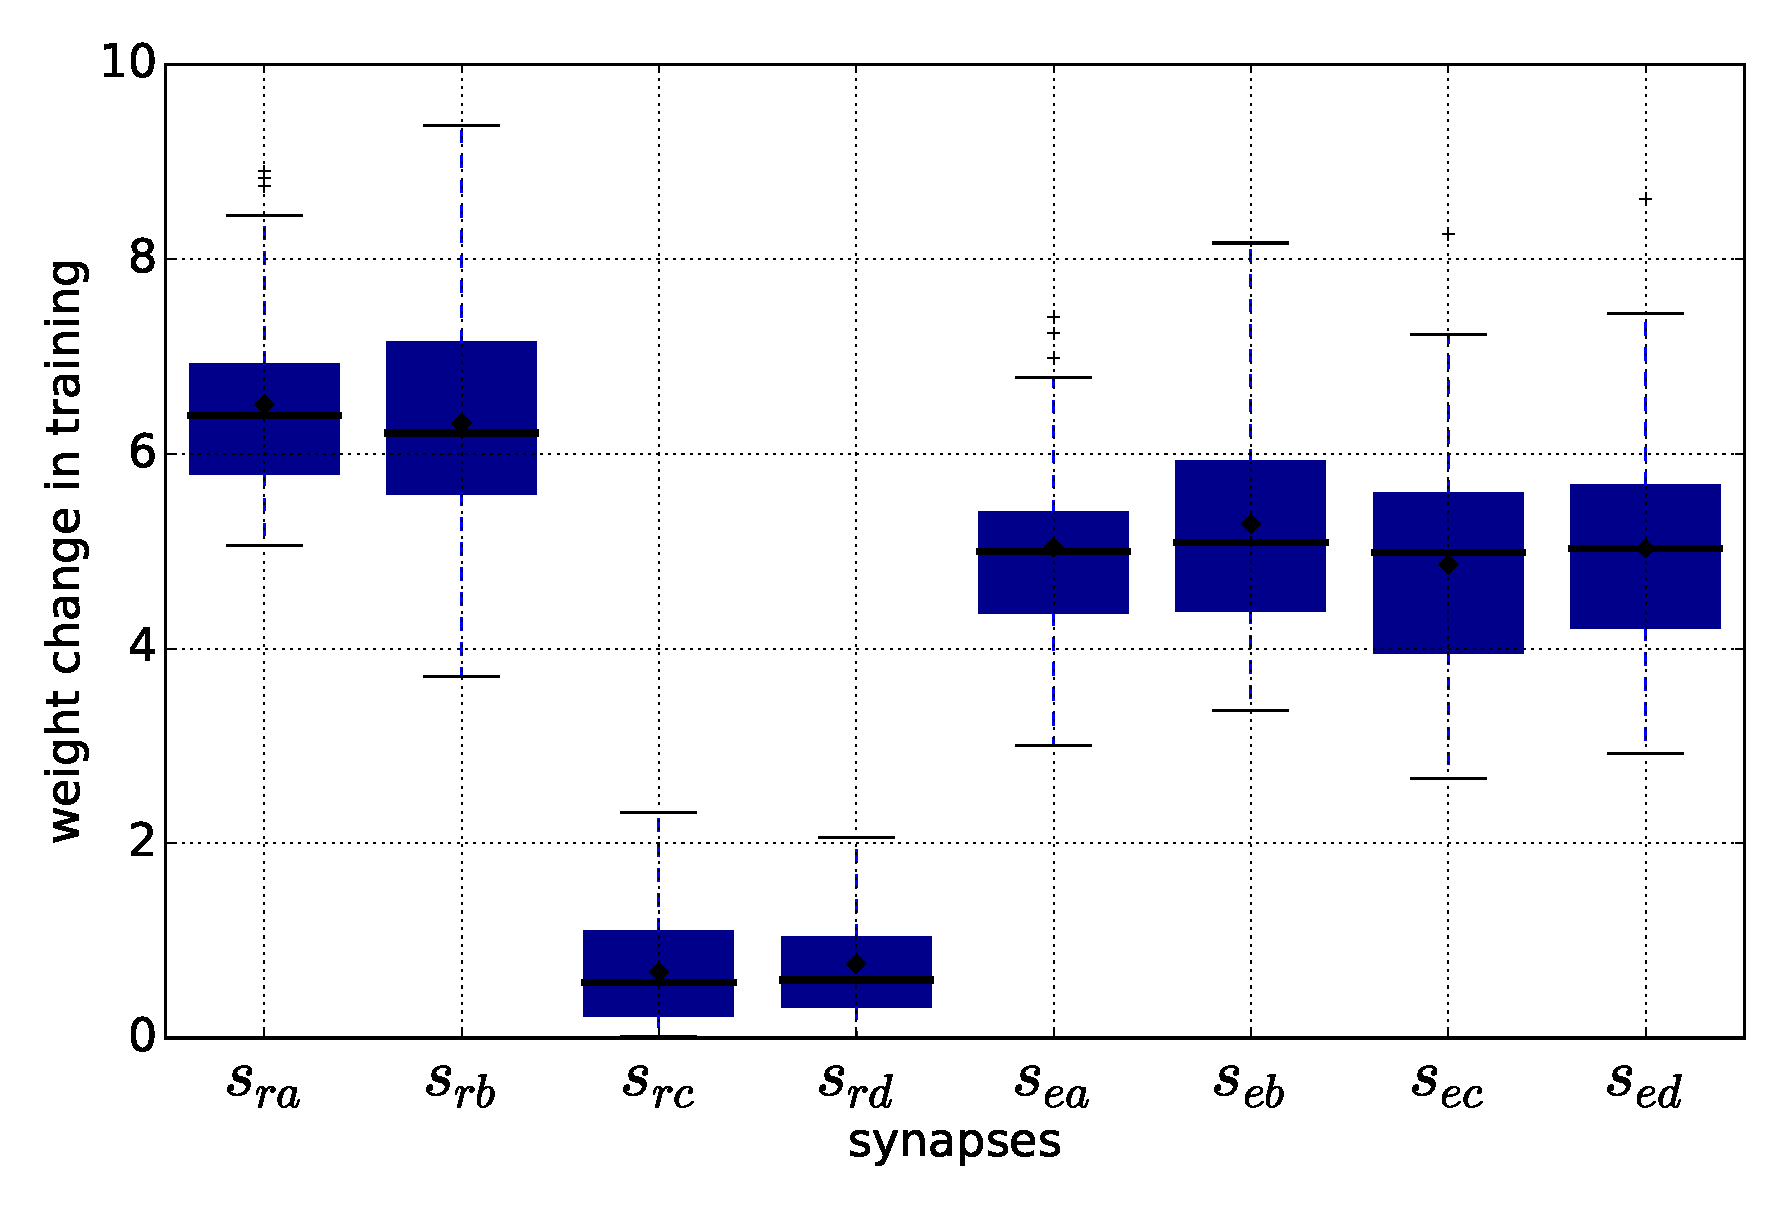
\includegraphics[width=\textwidth]{pruning_result_rpe.eps}
\caption{Weight change in training for input-hidden synapses (100 observations, RPE example).}
\label{fig:examples:pruning_result_rpe}
\end{figure}

Additionally, synapses responsible for \textit{rule} ($ s_{ra} $ and $ s_{rb} $) have a greater mean significance than the synapses connected with the \textit{exception} neuron ($ s_{e*} $).

\section{Michalski's Trains} \label{sec:example_trains}
The train problem was originally introduced in \citep{michalski}. The task was to determine concise decision rules distinguishing between two sets of trains (Eastbound and Westbound). In \citep{mozer_smolensky}, they presented a simplified version illustrated in \cref{fig:examples:dataset_train}.

\begin{figure}[H]
\centering
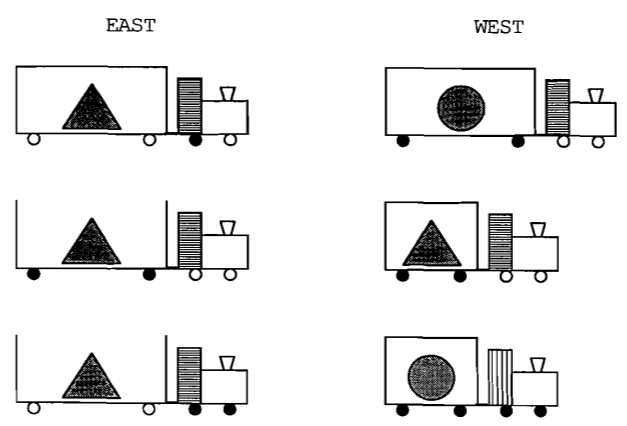
\includegraphics[width=0.7\textwidth]{train_problem}
\caption{Michalski's train problem.}
\label{fig:examples:dataset_train}
\end{figure}

Each train is described by $ 7 $ binary features listed in \cref{tab:examples:train_features}.

\begin{table}[H]
\centering
\begin{tabular}{|c|l|c|c|}
\hline
\multicolumn{2}{|c|}{feature} & \textit{encoded as \textbf{0}} & \textit{encoded as \textbf{1}} \\ \hline \hline
0 & car length                & long                  & short                 \\ \hline
1 & car type                  & open                  & closed                \\ \hline
2 & cabin pattern             & vertical lines        & horizontal lines      \\ \hline
3 & load shape                & triangle              & circle                \\ \hline
4 & color of trailer wheels   & white                 & black                 \\ \hline
5 & color of first car wheel  & white                 & black                 \\ \hline
6 & color of second car wheel & white                 & black                 \\ \hline
\end{tabular}
\caption{Features describing a train.}
\label{tab:examples:train_features}
\end{table}

Having \cref{tab:examples:train_features} we can encode the trains shown in \cref{fig:examples:dataset_train} into feature vectors as follows in \cref{tab:examples:train_feature_vectors}.

\begin{table}[H]
\centering
\begin{tabular}{|l|c|l|c|}
\hline
\multicolumn{2}{|c|}{\textit{class EAST}} & \multicolumn{2}{c|}{\textit{class WEST}} \\ \hline
east 1    & $ [0, 1, 1, 0, 0, 0, 1]^T $   & west 1   & $ [0, 1, 1, 1, 1, 0, 0]^T $   \\ \hline
east 2    & $ [0, 0, 1, 0, 1, 0, 0]^T $   & west 2   & $ [1, 1, 1, 0, 1, 0, 0]^T $   \\ \hline
east 3    & $ [0, 0, 1, 0, 0, 1, 1]^T $   & west 3   & $ [1, 1, 0, 1, 1, 1, 1]^T $   \\ \hline
\end{tabular}
\caption{Feature vectors for different train types.}
\label{tab:examples:train_feature_vectors}
\end{table}

The task is to determine the minimal number of input features capable of the east-west classification based on the six possible types in \cref{tab:examples:train_feature_vectors} (or in \cref{fig:examples:dataset_train}).

The hypothesis is that the pruning algorithm should select the needed features by eliminating unimportant input-hidden synapses. Looking at \cref{fig:examples:dataset_train} one of the solutions could be keeping features $ (0, 3) $, because the shape of the load together with the length of the car is enough to distinguish \textit{west} trains from \textit{east} trains. Another solution, for example, is keeping the car length, car type and color of the second car wheel - features $ (0, 1, 6) $.

To test our pruning algorithm on this feature selection task, a dataset of $ 6000 $ samples ($ 3000 $ west and $ 3000 $ east trains) was generated. The three possible train types for each class (\cref{fig:examples:dataset_train}) are equally distributed among the samples, meaning we have $ 1000 $ samples of each train type.

As shown in \citep{mozer_smolensky}, one hidden neuron is enough to learn this problem, hence we started with the network structure $ [7, 1, 2] $. The experiment parameters are listed in \cref{tab:examples:train_settings}.

\begin{table}[H]
\centering
\scalebox{0.95}{
\begin{tabular}{|l|c|l|c|l|c|}
\hline
\multicolumn{2}{|c|}{\textit{initial network}} & \multicolumn{2}{c|}{\textit{learning parameters}} & \multicolumn{2}{c|}{\textit{pruning parameters}} \\ \hline
structure             & {[}7, 1, 2{]}          & learning rate                  & 0.3              & required accuracy             & 1.0             \\ \hline
n synapses            & 9                      & number of epochs               & 100               & retrain                       & True             \\ \hline
transfer fcn          & sigmoid                & minibatch size                 & 1                & retraining epochs             & 10               \\ \hline
\end{tabular}}
\caption{Experiment settings for the train example.}
\label{tab:examples:train_settings}
\end{table}

We ran $ 100 $ observations of the experiment and considered the features that were not cut out, as a result of a single experiment.

\begin{figure}[H]
\centering
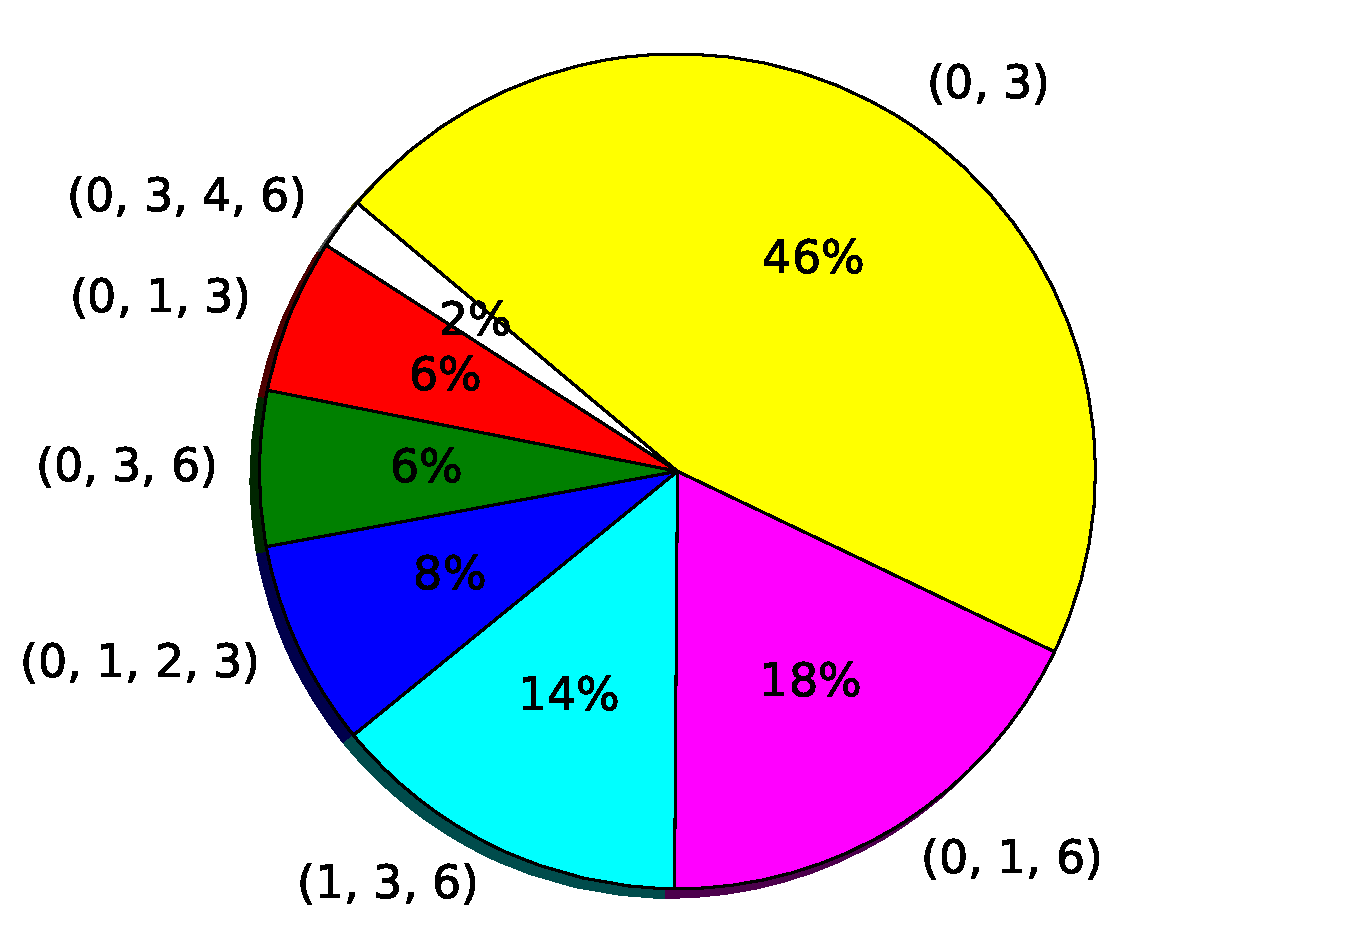
\includegraphics[width=0.7\textwidth]{pruning_result_pie_train.eps}
\caption{Results of feature selection by the pruning algorithm (train example). The labels corresponds with feature indices in \cref{tab:examples:train_features}.}
\label{fig:examples:pruning_result_pie_train}
\end{figure}

The result pie in \cref{fig:examples:pruning_result_pie_train} shows that the pruning algorithm found the best possible solution ($ (0, 3) $ - the car length and the load shape) in $ 46\% $ of the cases. We can regard the $ (0, 1, 6) $ and $ (1, 3, 6) $ as another (not best but also good) solutions. The rest we consider as fail cases, as all of them include features $ (0, 3) $ and the other features are redundant. To sum it up, we got a perfect solution: $ 46\% $; a good solution: $ 32\% $; a bad solution: $ 22\% $.

\section{Handwritten Digits (MNIST)} \label{sec:example_mnist}
The MNIST (Modified National Institute of Standards and Technology) database \citep{wiki:mnist} is a large database of handwritten digits that is widely used for training and testing methods in the field of machine learning. 

The dataset was downloaded from \citep{online:mnist}. Some of the digits were written by employees of American Census Bureau \citep{online:census} and some by students of an American high school. In total $ 70000 $ samples were collected. Examples are shown in \cref{fig:examples:dataset_mnist}.

\begin{figure}[H]
\centering
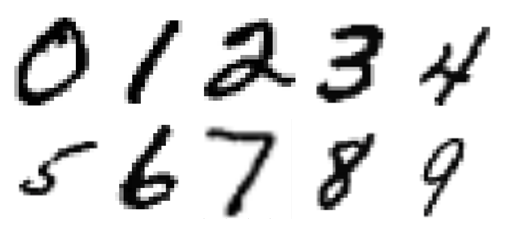
\includegraphics[width=0.9\textwidth]{dataset_mnist}
\caption{Examples of MNIST dataset.}
\label{fig:examples:dataset_mnist}
\end{figure}

Each sample is a grayscale image (normalised to $ [0, 1] $) of size $ 28x28 $ pixels. This gives row-by-row a vector of $ 784 $ features. The data was splitted into a training set of $ 50000 $ samples, a validation set of $ 10000 $ samples and a testing set of $ 10000 $ samples.

From \citep{online:mnist} we know the problem can be learnt by a feedforward network with one hidden layer up to high accuracy ($ 98-99\% $). The first task is to achieve similar results with the implemented neural net framework. We tested the following learning settings (\cref{tab:examples:mnist_training_settings}).

\begin{table}[H]
\centering
\begin{tabular}{|l|c|l|c|}
\hline
\multicolumn{2}{|c|}{\textit{network parameters}} & \multicolumn{2}{c|}{\textit{learning parameters}} \\ \hline
structure               & {[}784, 20, 10{]}       & learning rate                  & 0.3              \\ \hline
n synapses              & 15880                   & number of epochs               & 100              \\ \hline
transfer function       & sigmoid                 & batch size               & 10              \\ \hline
\end{tabular}
\caption{Settings for training a dense feedforward net on the MNIST dataset.}
\label{tab:examples:mnist_training_settings}
\end{table}

The training results are summarized in \cref{tab:examples:mnist_training_results}. A confusion matrix for the testing data is given in \cref{fig:examples:mnist_cm}.

\begin{table}[H]
\centering
\begin{tabular}{|l|c|c|}
\hline
                       & \multicolumn{1}{l|}{\textit{accuracy}} & \multicolumn{1}{l|}{\textit{MSE}} \\ \hline
\textit{training data} & $ 97.2\% $                                      & 0.526                                 \\ \hline
\textit{testing data}  & $ 94.3\% $                                      & 1.025                                 \\ \hline
\end{tabular}
\caption{Training results on MNIST dataset.}
\label{tab:examples:mnist_training_results}
\end{table}

\begin{figure}[H]
\centering
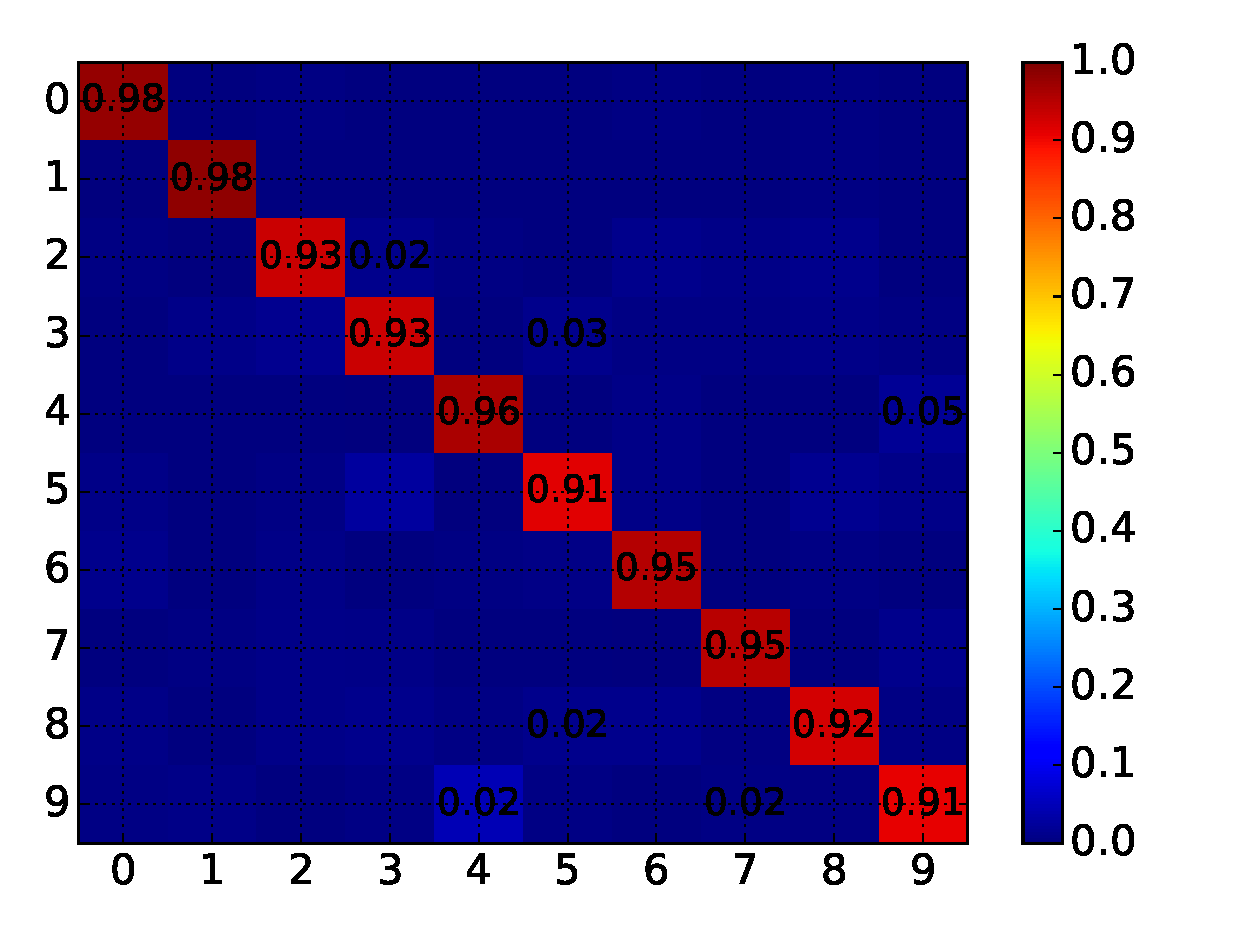
\includegraphics[width=0.7\textwidth]{mnist_training_result_cm.eps}
\caption{Confusion matrix (MNIST, testing data).}
\label{fig:examples:mnist_cm}
\end{figure}

In the following, the pruning method is analysed on networks trained on the MNIST database. Parameters of the learning-pruning procedure are listed in \cref{tab:examples:mnist_settings}.

\begin{table}[H]
\centering
\scalebox{0.9}{
\begin{tabular}{|l|c|l|c|l|c|}
\hline
\multicolumn{2}{|c|}{\textit{initial network}} & \multicolumn{2}{c|}{\textit{learning parameters}} & \multicolumn{2}{c|}{\textit{pruning parameters}} \\ \hline
structure             & {[}784, 20, 10{]}          & learning rate                  & 0.3              & required accuracy             & 0.97             \\ \hline
n synapses          & 15800                & number of epochs               & 30               & retrain                       & True             \\ \hline
transfer fcn          & sigmoid                & minibatch size                 & 10                & retraining epochs             & 10               \\ \hline
\end{tabular}}
\caption{Experiment settings for the MNIST example.}
\label{tab:examples:mnist_settings}
\end{table}

The hypothesis is that the initial number of synapses in the network ($ 15800 $) is redundant, as well as the number of features ($ 784 $). In \cref{fig:examples:pruning_process_mnist} we can see a selected observation of the pruning process. The number of synapses was reduced to $ 1259 $ and the number of used features to $ 465 $, while the classification accuracy was kept on $ 97\% $. The pruning procedure finished in $ 424 $ pruning steps (explained in [PA]).

\begin{figure}[H]
\centering
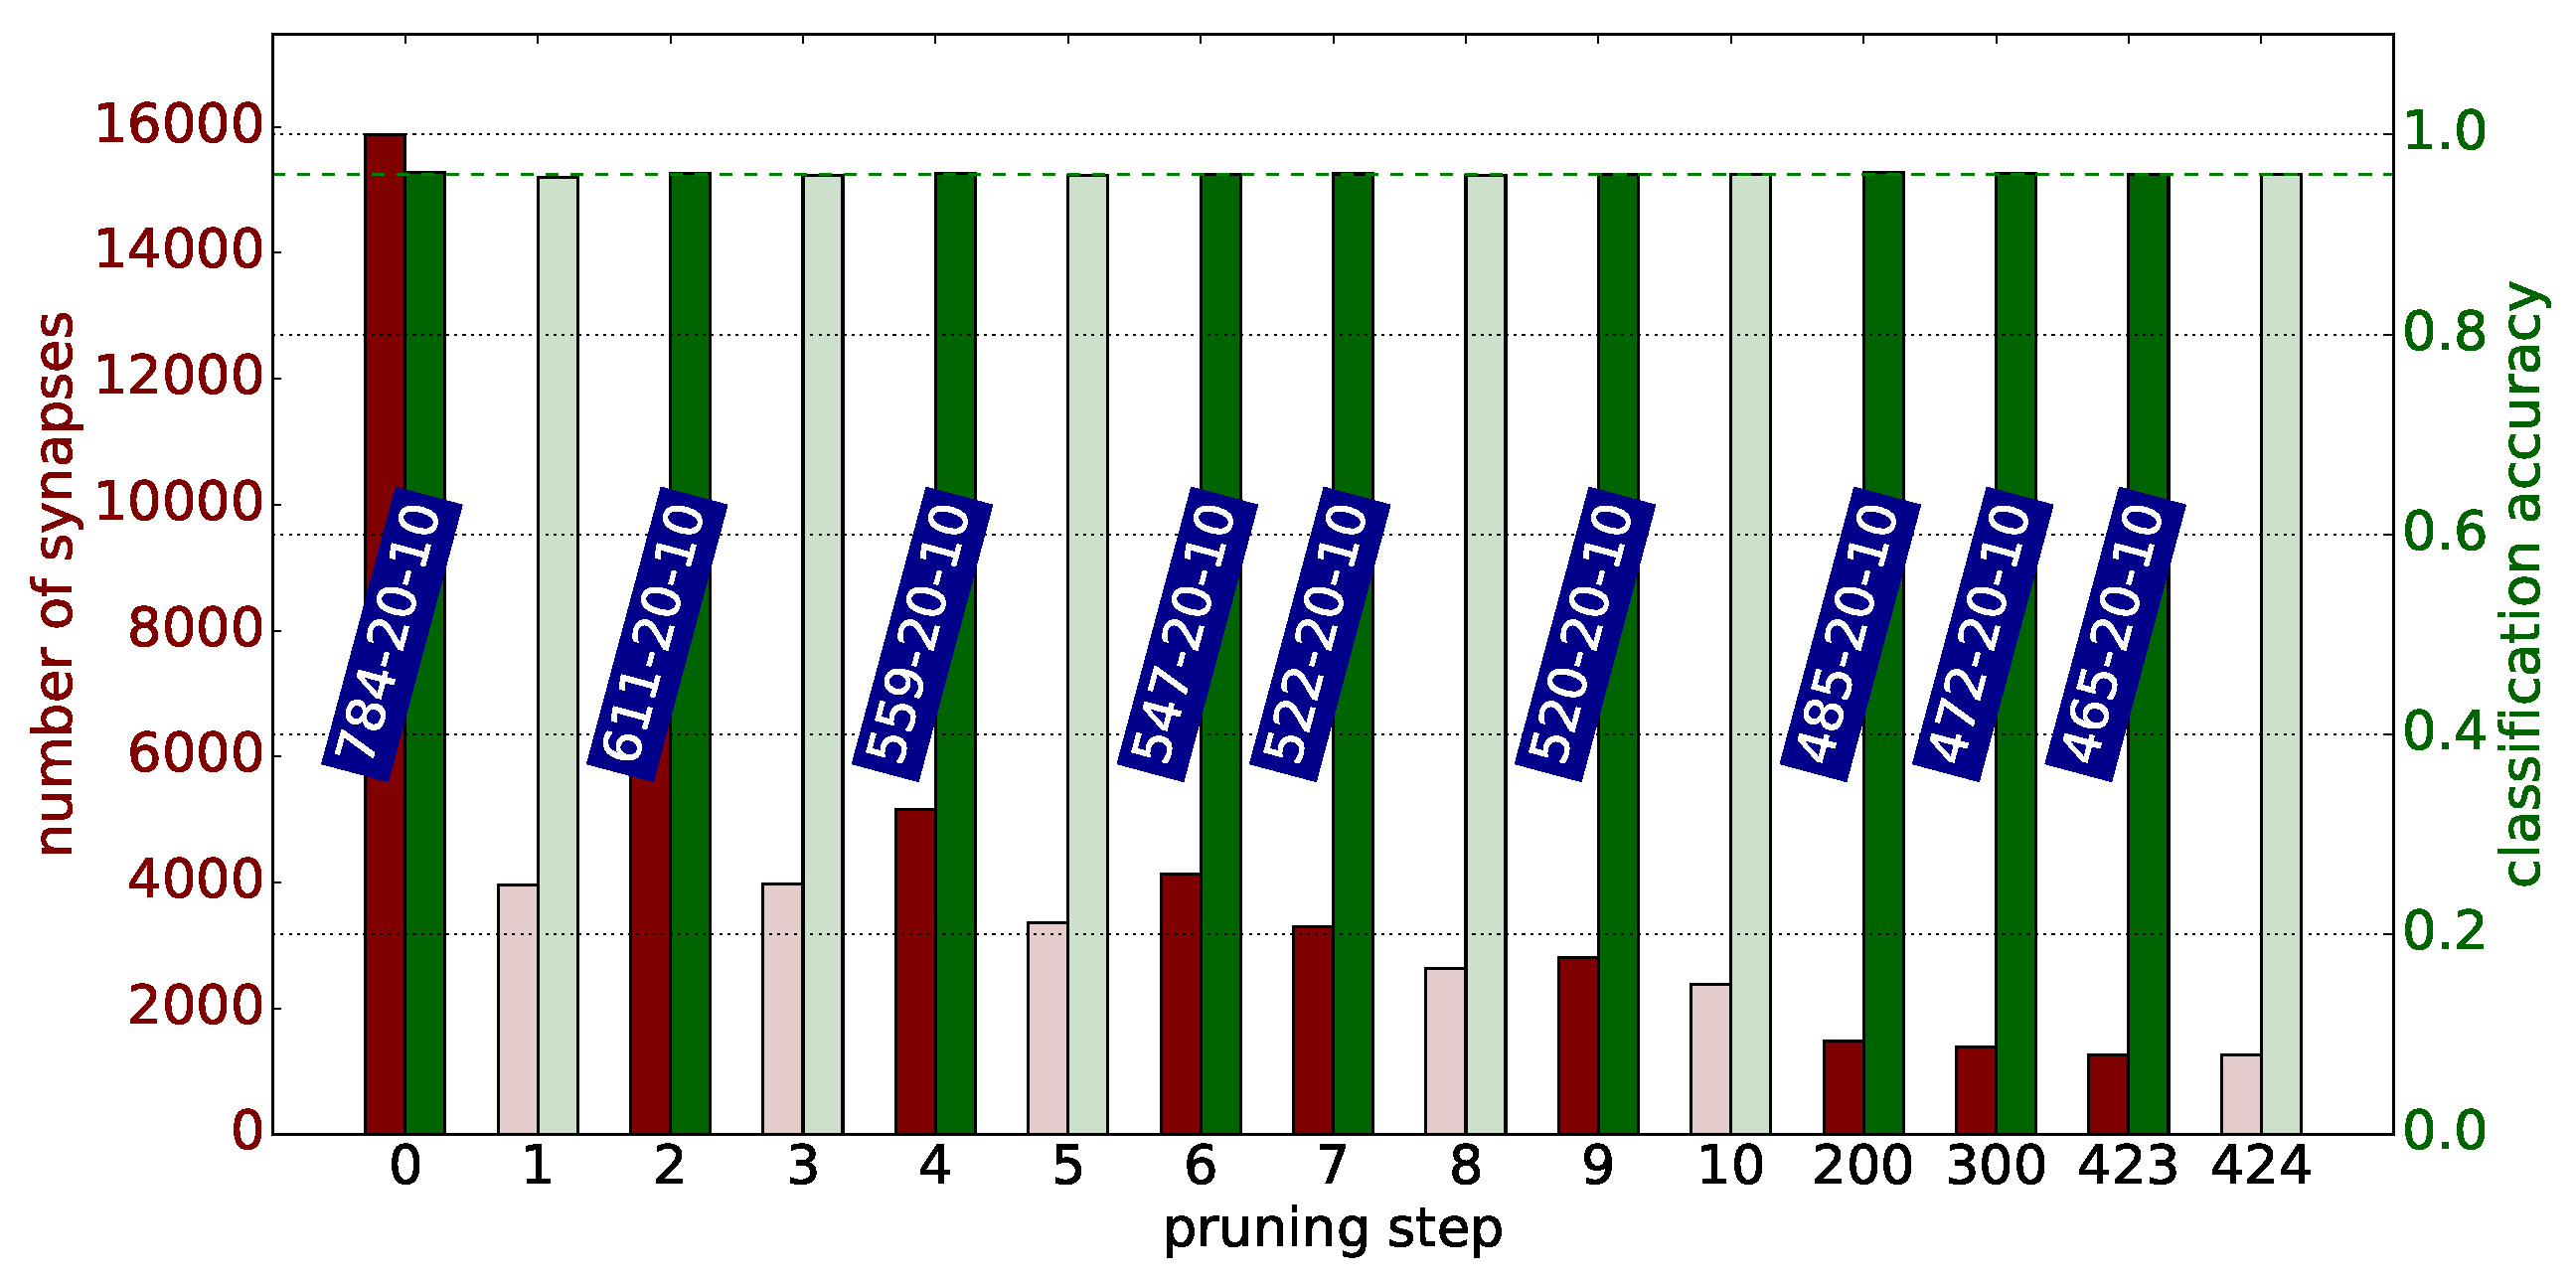
\includegraphics[width=\textwidth]{pruning_process_mnist.eps}
\caption{Illustration of the pruning procedure applied on MNIST dataset (selected observation). Required accuracy: $ 97\% $.}
\label{fig:examples:pruning_process_mnist}
\end{figure}

In \cref{fig:examples:evaluation_time_mnist}, we can see a comparison of the evaluation time. We compare a fully-connected (initial) network to a pruned one. Bars are given for the three data groups (training: $ 50000 $ samples, validation: $ 10000 $ samples, testing: $ 10000 $ samples). The processing time was reduced by nearly half after the pruning, which led to a reduction of weight matrix dimension (see [SHRINK]).

\begin{figure}[H]
\centering
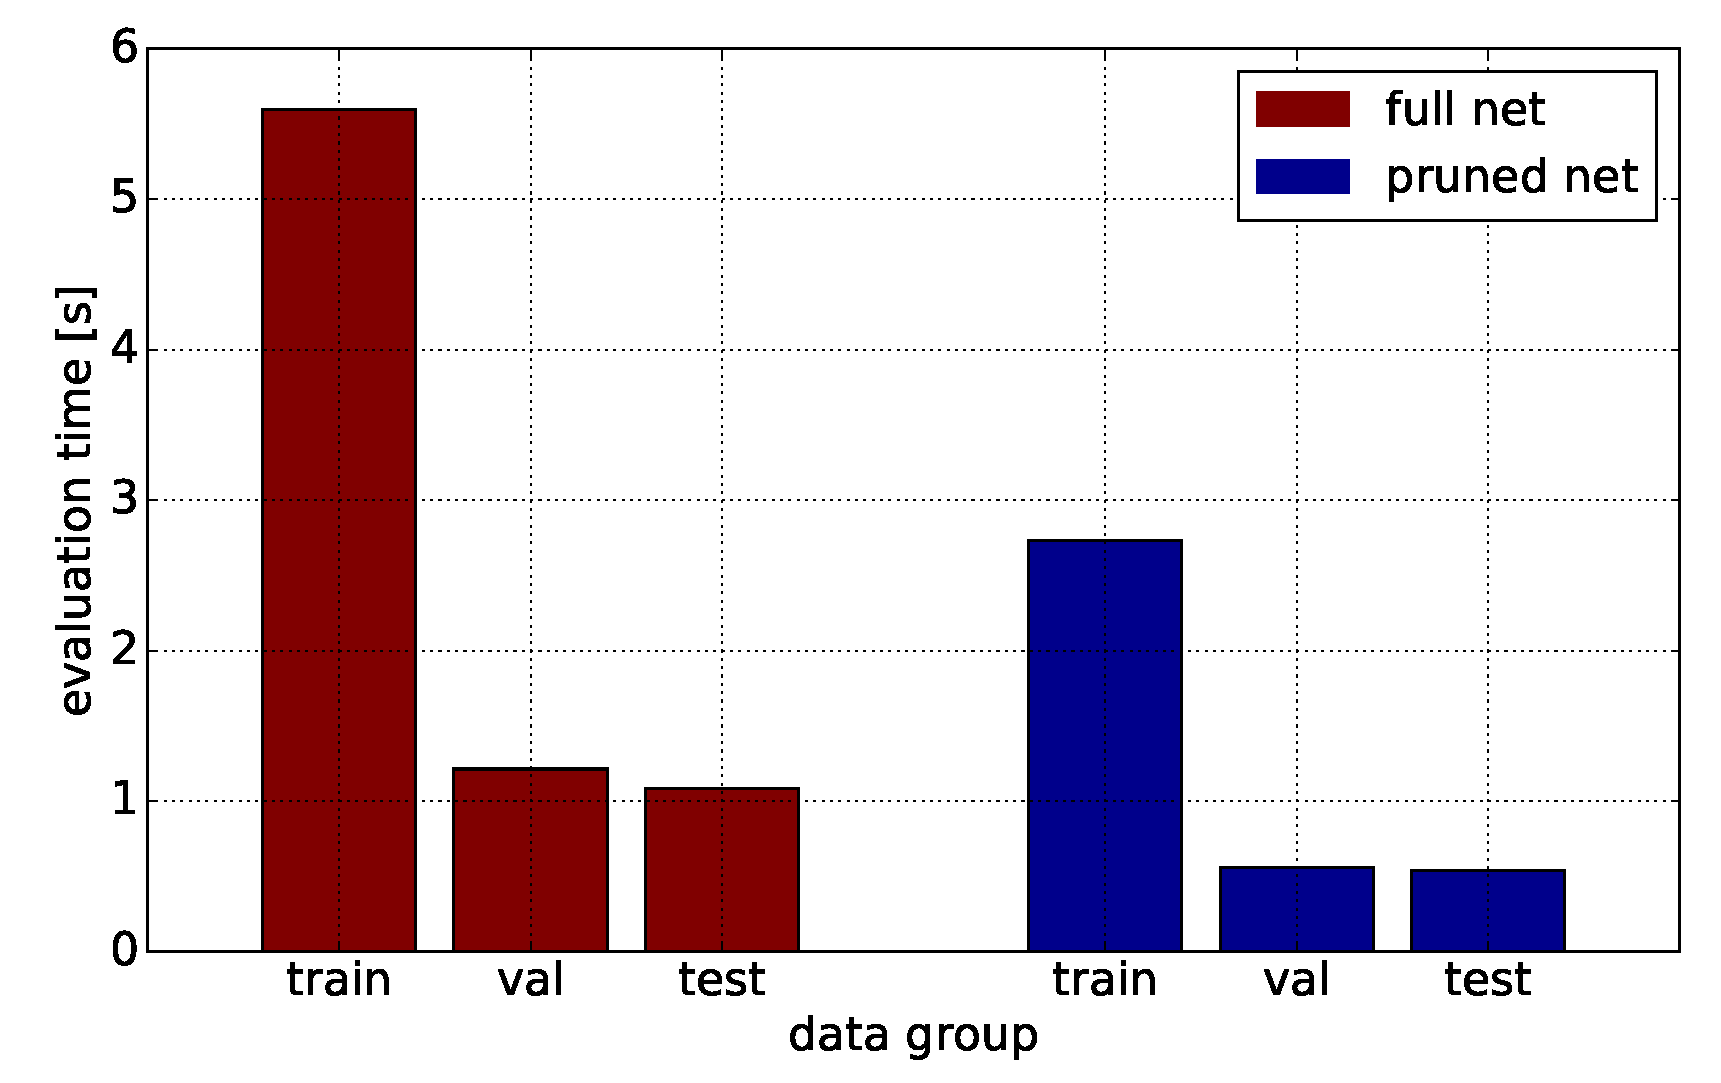
\includegraphics[width=0.8\textwidth]{evaluation_time_mnist.eps}
\caption{Evaluation (accuracy and error computation) time for all data groups (pruned vs. full net).}
\label{fig:examples:evaluation_time_mnist}
\end{figure}

 \cref{fig:examples:mnist_pruning_vs_req_acc} gives the statistics by running 10 observations of the pruning procedure for several values of required classification accuracy. We observed the number of synapses (red axis) and used features after pruning (blue axis).

\begin{figure}[H]
\centering
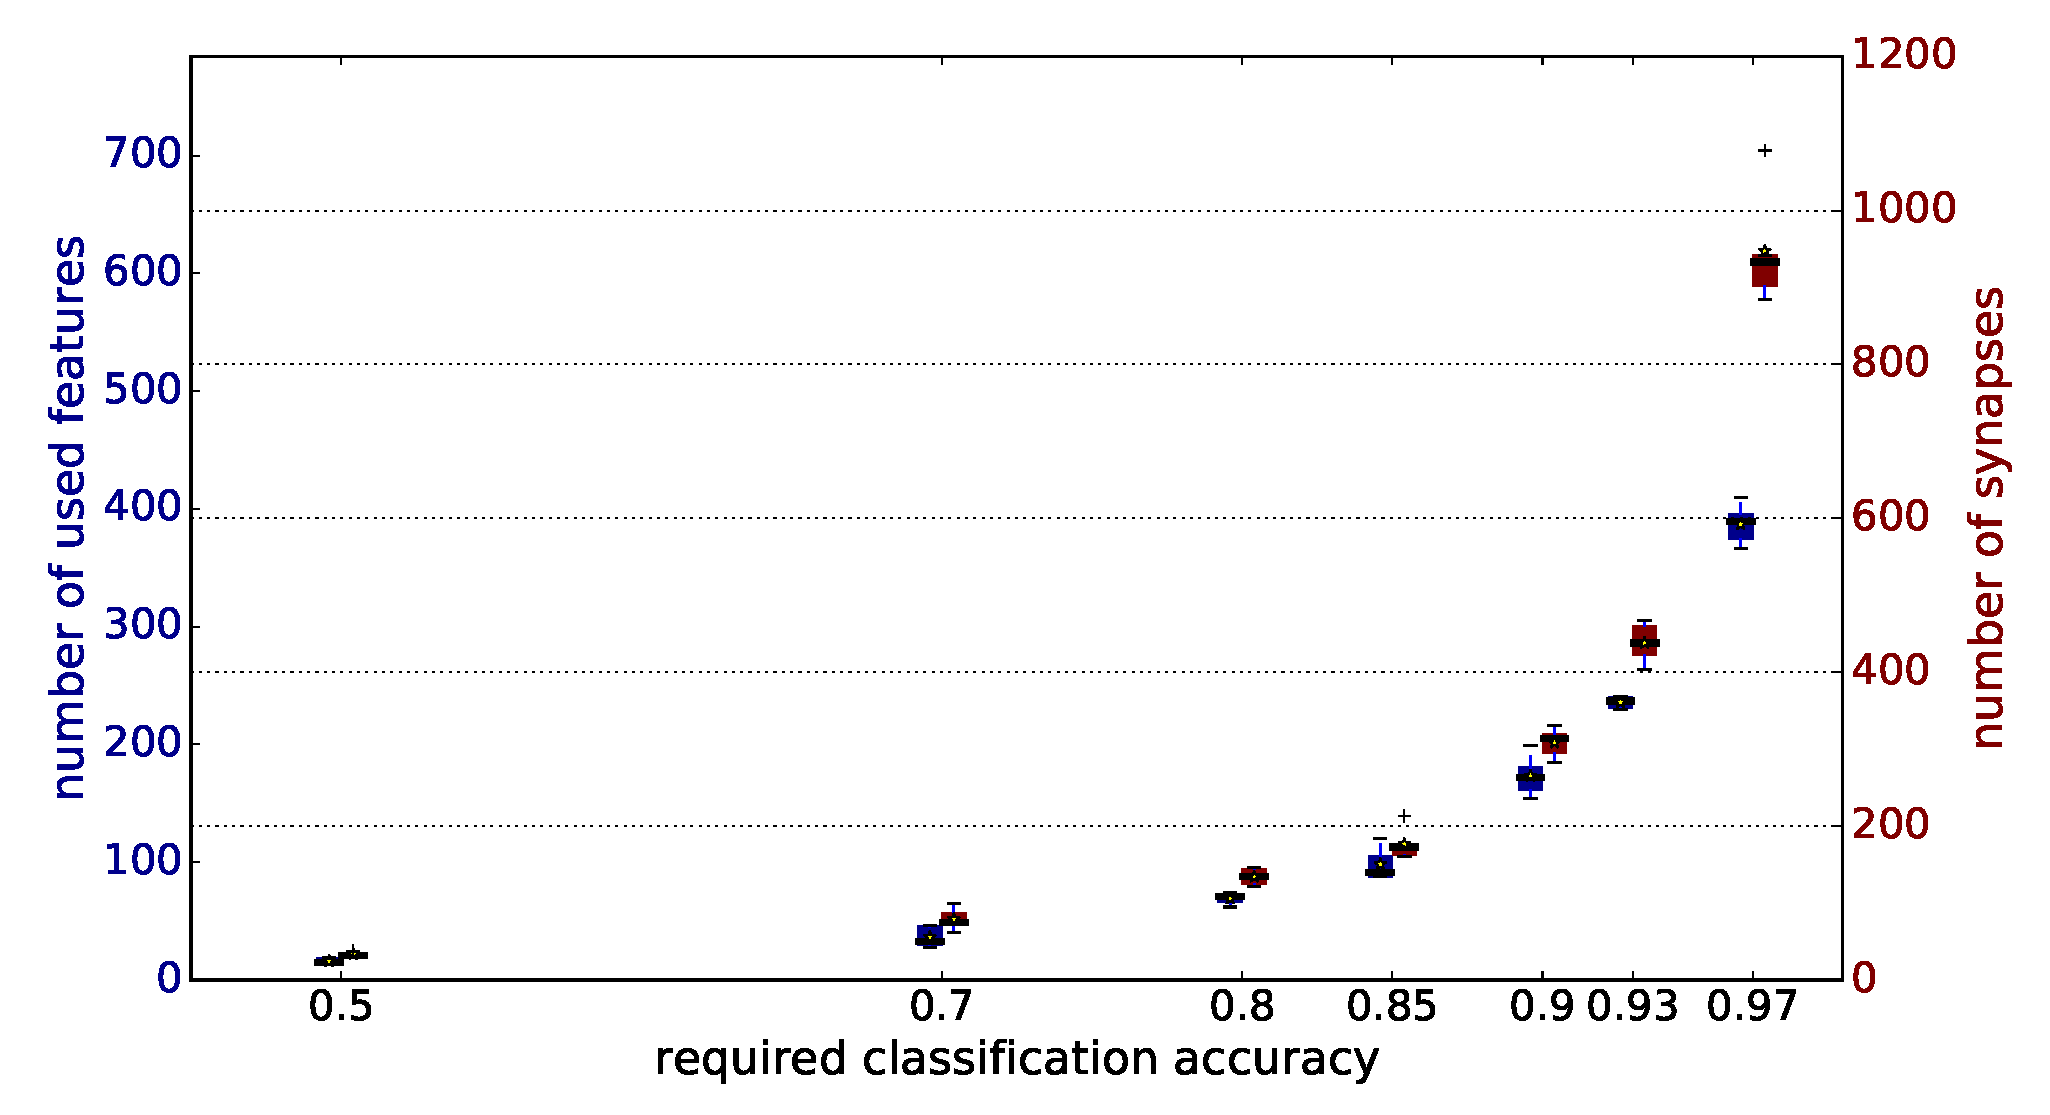
\includegraphics[width=\textwidth]{pruning_result_vs_req_acc.eps}
\caption{Minimal number of features and synapses to get required classification accuracy (MNIST data).}
\label{fig:examples:mnist_pruning_vs_req_acc}
\end{figure}

The results show that \textit{less than a tenth} of the synapses and \textit{about a half} of the features are needed to keep the maximal classification accuracy ($ 97\% $). It is also worth saying that the MNIST dataset can be learnt to $ 50\% $ using only $ 20 $ features and a network with $ 38 $ synapses. In the following, these two results are further analysed.

\subsubsection*{Minimal MNIST network}
At first, we focus on a pruned network capable of MNIST classification with accuracy of $ 50\% $ (\cref{fig:examples:pruned_net_mnist_05}). This example is simple enough to show the feature selection method described in [ref FS].

\begin{figure}[H]
\centering
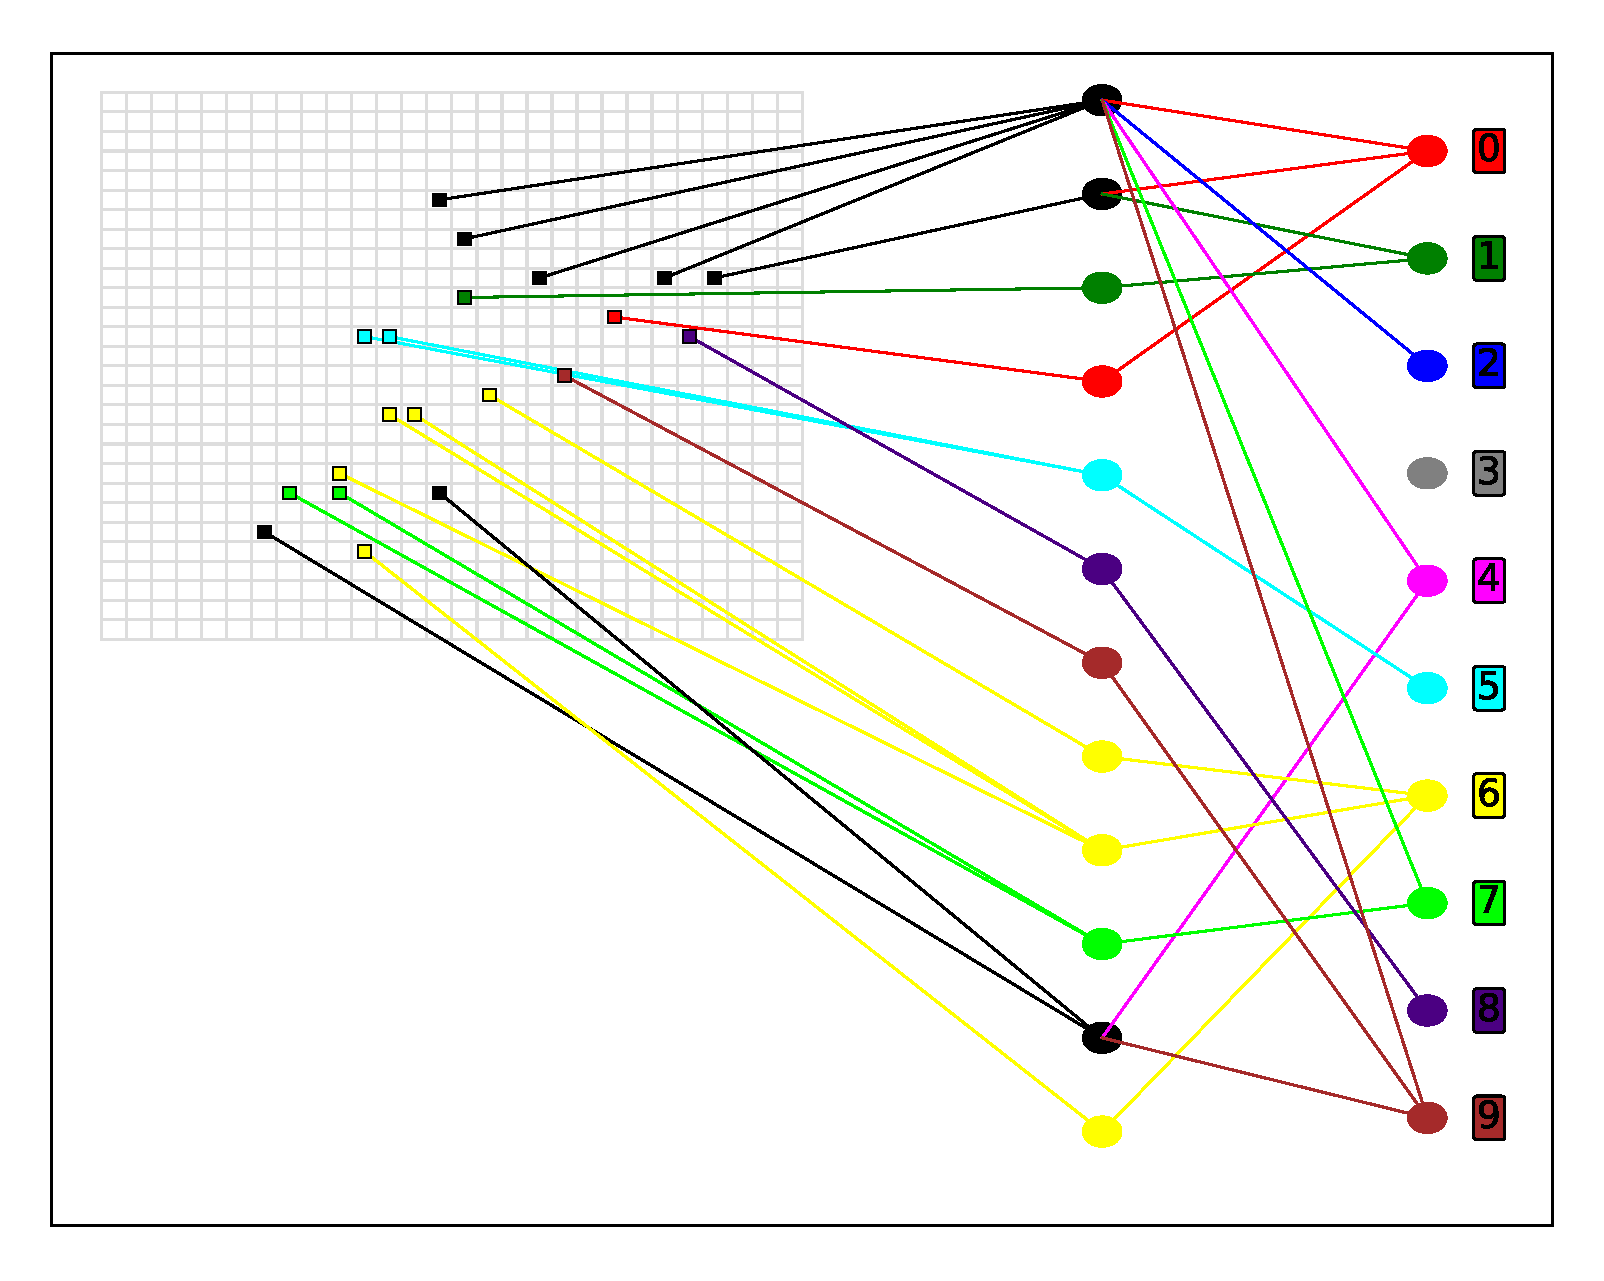
\includegraphics[width=0.7\textwidth]{pruned_net_mnist_05.eps}
\caption{Result of network pruning and path tracking, MNIST data, accuracy: $ 50\% $.}
\label{fig:examples:pruned_net_mnist_05}
\end{figure}

Each class (digit in this case) has its color. If a hidden unit has one output connection only, it inherits the color of the class it is connected to. The features (pixels of the $ 28x28 $ image) are then colored in the same way. If a hidden unit influences more than one class, it is blacked. All features connected to a black hidden unit are then blacked as well, as they also affects more than one class.

\begin{figure}[H]
\centering
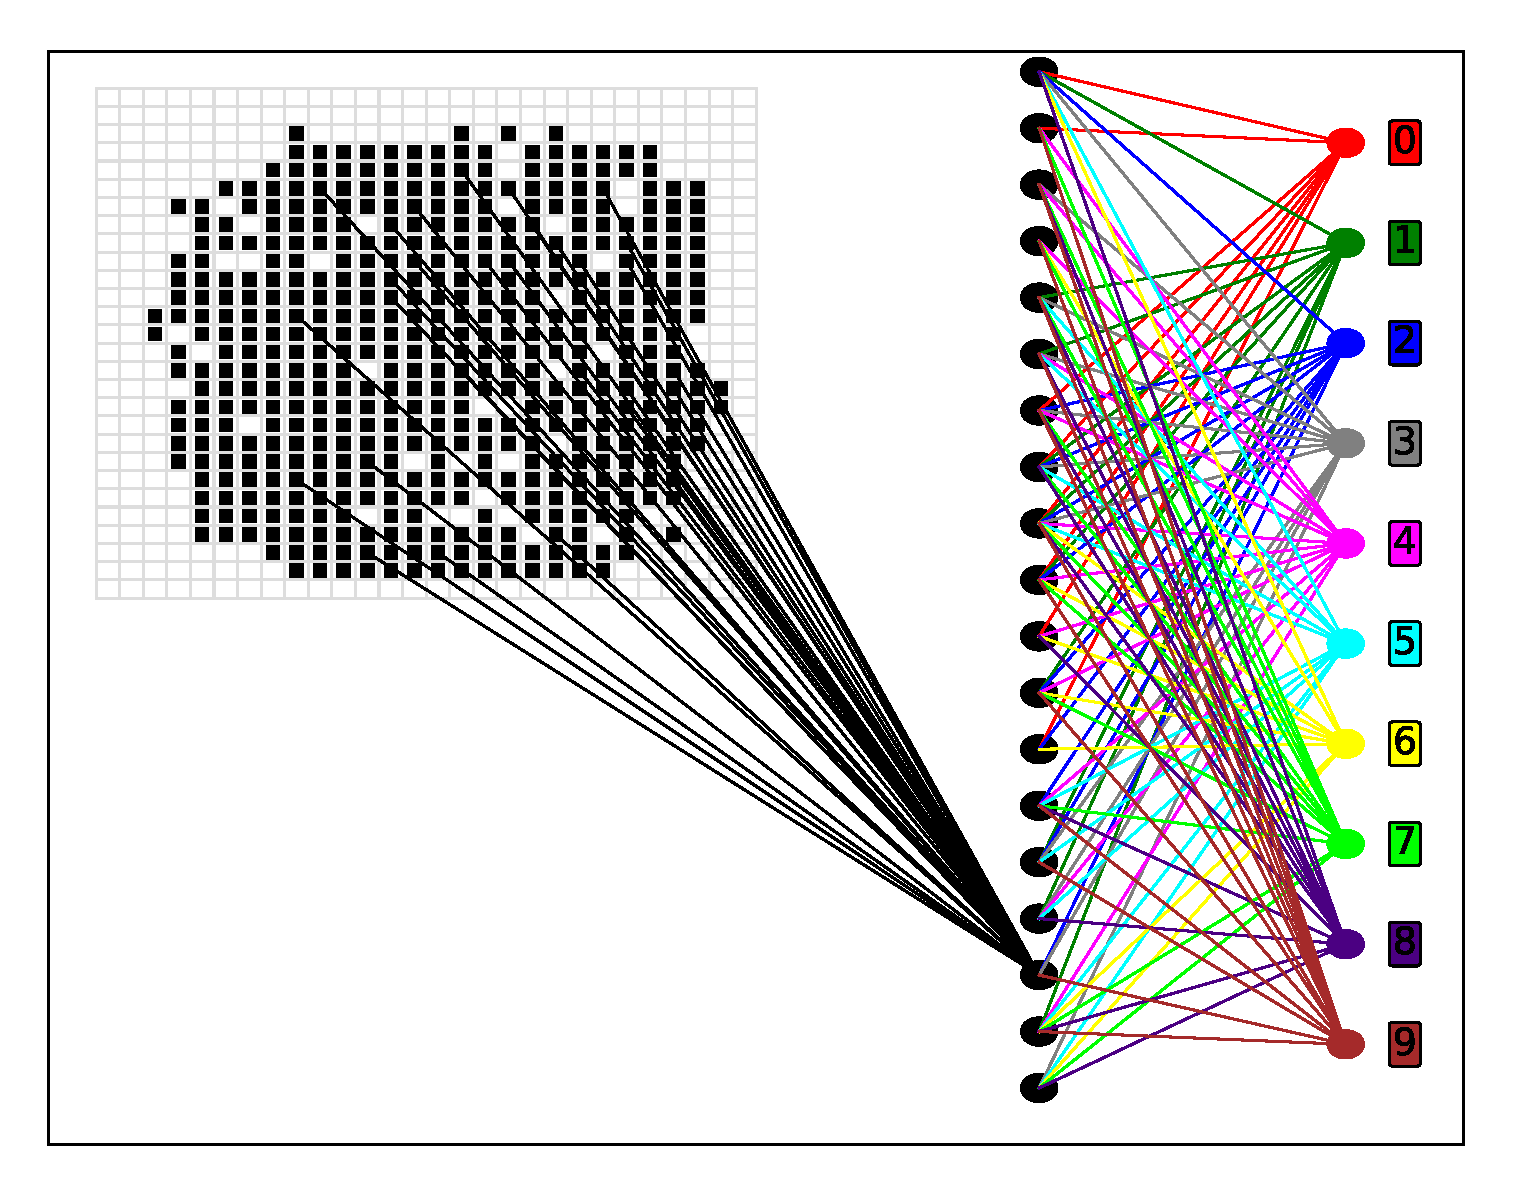
\includegraphics[width=0.7\textwidth]{pruned_net_mnist_097.eps}
\caption{Result of network pruning and path tracking (shown $ 17^{th} $ hidden neuron only), MNIST data, accuracy: $ 97\% $.}
\label{fig:examples:pruned_net_mnist_097}
\end{figure}

A pruned network capable of $ 97\% $ accurate classification is visualized in \cref{fig:examples:pruned_net_mnist_097}. To make the figure clearer, only synapses coming to the $ 17^{th} $ hidden unit are drawn between the input and hidden layer.

We can see that each of the features affects more than one class in this case. Therefore we better use the visualization in \cref{fig:examples:fs_mnist}. 

\begin{figure}[H]
\centering
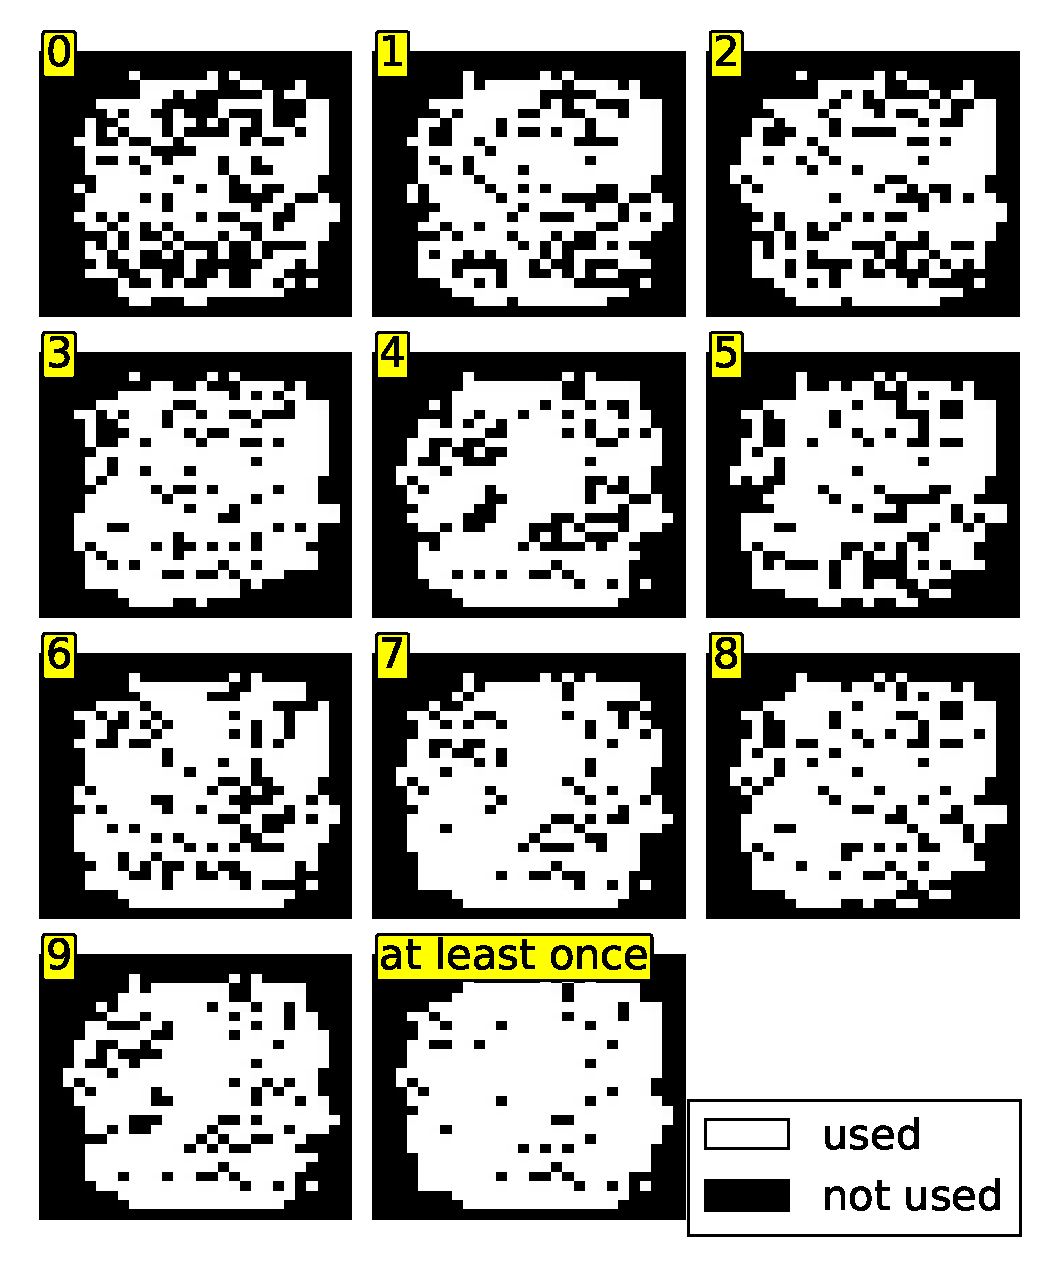
\includegraphics[width=0.95\textwidth]{fs_mnist.eps}
\caption{Used features for individual classes, MNIST data, accuracy: $ 97\% $.}
\label{fig:examples:fs_mnist}
\end{figure}

Knowing all the remaining synapses are important for classification, we can track tha paths from individual classes to features. This way we distinguish features connected to a selected class from those that do not affect that class. \cref{fig:examples:fs_mnist} shows important features for each class (digit) separately. Note that the \textit{at-least-once} subplot corresponds to the features shown in \cref{fig:examples:pruned_net_mnist_097}. It shows all features used by at least one class.

Some more ideas about path tracking in pruned networks are further discussed in \cref{sec:future_work}.

\section{Phonemes (Speech Data)} \label{sec:example_speech}
The process of speech data gathering is described in \cref{sec:speech_data_gathering}. The dataset generation process has three parameters: \texttt{border\textunderscore size} ($ bs $), \texttt{context\textunderscore size} ($ cs $) and \texttt{n\textunderscore samples} ($ ns $).

In this example, we first try to find optimal parameter settings, which would lead to a maximal trainability. The general rule is the more samples the better trainability, therefore we fix $ ns = 1000 $ and determine the other parameters at first. See \cref{tab:app:speech_datasets} for details of all generated datasets differing in $ bs $ and $ cs $. It reveals that phoneme \texttt{"F"} does not have enough occurrences (less than $ ns = 1000 $) in the data, and of course the number of occurrences decreases with growing $ bs $. For $ bs >= 6 $ even more phonemes (\texttt{"D"}, \texttt{"F"},\texttt{"N"}, \texttt{"Q"}, \texttt{"R"}, \texttt{"T"}) have less than $ 1000 $ occurrences.

\cref{tab:examples:speech_bs_cs_determination} shows the experiment settings.

\begin{table}[H]
\centering
\begin{tabular}{|l|c|l|c|}
\hline
\multicolumn{2}{|c|}{experiment settings}   & \multicolumn{2}{c|}{learning parameters} \\ \hline
n observations    & 5                       & learning rate            & 0.1           \\ \hline
observed value    & MSE' (\cref{eq:mse_})    & n epochs                 & 50            \\ \hline
network structure & {[}$ 40 \cdot (2cs+1) $, 50, 40{]} & batch size               & 10            \\ \hline
\end{tabular}
\caption{Speech dataset: experiment settings for determination of optimal $ bs $ and $ cs $.}
\label{tab:examples:speech_bs_cs_determination}
\end{table}

We ran $ 5 $ observations of a simple network training for every combination of $ bs \in [0, 5] $ and $ cs \in [0, 9] $. \cref{fig:examples:speech_bs_cs_test} shows average MSE' (see \cref{eq:mse_}) values. Complete results can be tracked in \cref{tab:app:speech_bs_cs_complete_results}.

\begin{figure}[H]
\centering
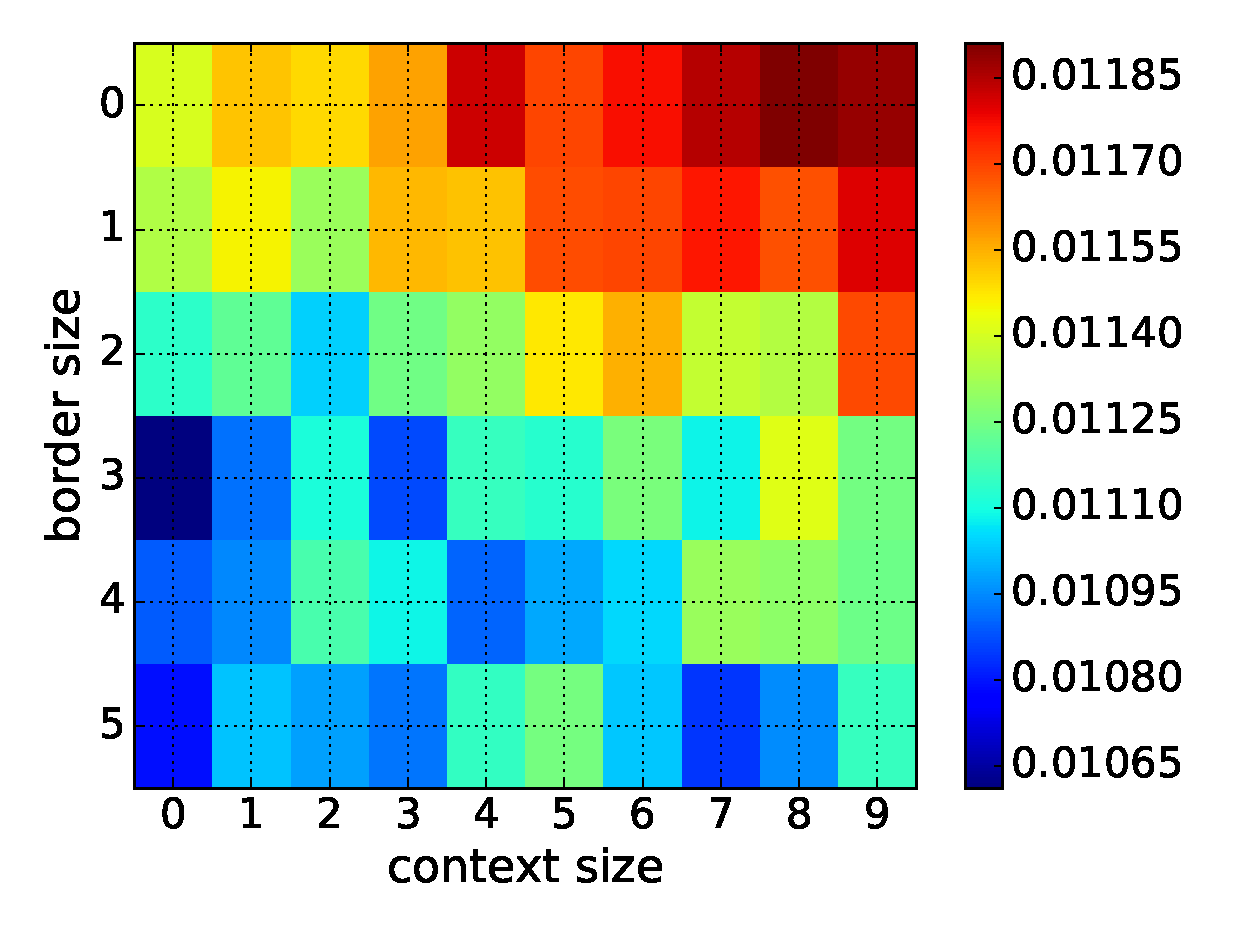
\includegraphics[width=0.8\textwidth]{speech_bs_cs_test.eps}
\caption{Test MSE' (\cref{eq:mse_}) for various parameters $ bs $ and $ cs $ ($ ns = 1000 $, 5 observations, see \cref{tab:app:speech_datasets}).}
\label{fig:examples:speech_bs_cs_test}
\end{figure}

The experiment result says that a bigger \texttt{context\textunderscore size} ($ cs > 2 $) does not go well together with a low \texttt{border\textunderscore size} ($ bs \leq 2 $). We can state that the \texttt{border\textunderscore size} should better be greater than two. Then the \texttt{context\textunderscore size} does not influence the trainability much. We must keep in mind that the experiment is too simple to give a reliable estimate (simple network structure, few training epochs), however, it gives an initial idea of a general trend, which is enough for the purposes of this work. For the experiments below we consider this settings:

\begin{itemize}
\item \texttt{border\textunderscore size}: $ bs = 3 $
\item \texttt{context\textunderscore size}: $ cs = 3 $
\item \texttt{n\textunderscore samples}: $ ns = 10000 $
\end{itemize}

\subsection*{Analysis of the Generated Speech Dataset}
The goal of this section is to show what kind of data we actually work with. In \cref{fig:examples:speech_example_sample_cs0} we can see one randomly selected sample for each phoneme. For a more illustrative view the context is cut out ($ cs = 0 $), hence we see $ 40 $ features corresponding to $ 40 $ frequency filters (see \cref{fig:methods:mfcc_filterbank}).

\begin{figure}[H]
\centering
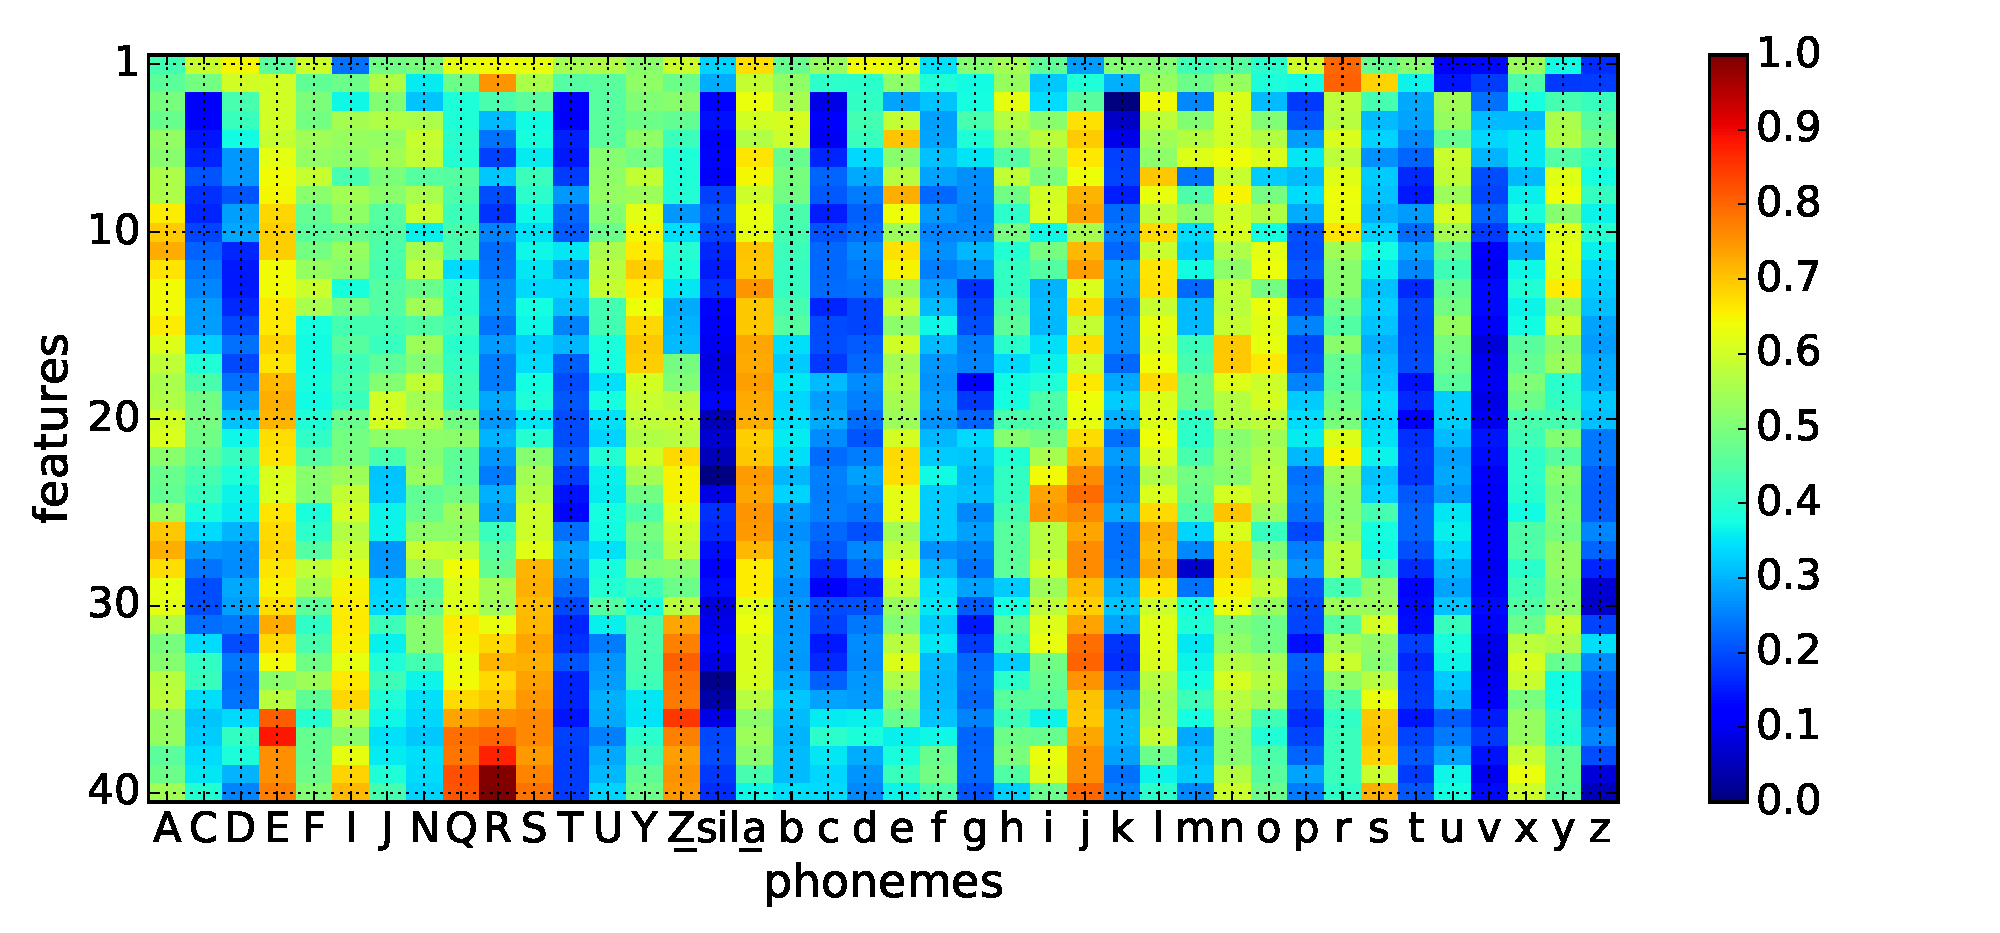
\includegraphics[width=\textwidth]{example_sample_10K_cs0_norm.eps}
\caption{Randomly selected sample for each phoneme, $ cs = 0 $.}
\label{fig:examples:speech_example_sample_cs0}
\end{figure}

\cref{fig:examples:speech_average_sample_cs0} shows an average feature vector out of $ 10000 $ samples for each phoneme. Here we can find some patterns.

\begin{figure}[H]
\centering
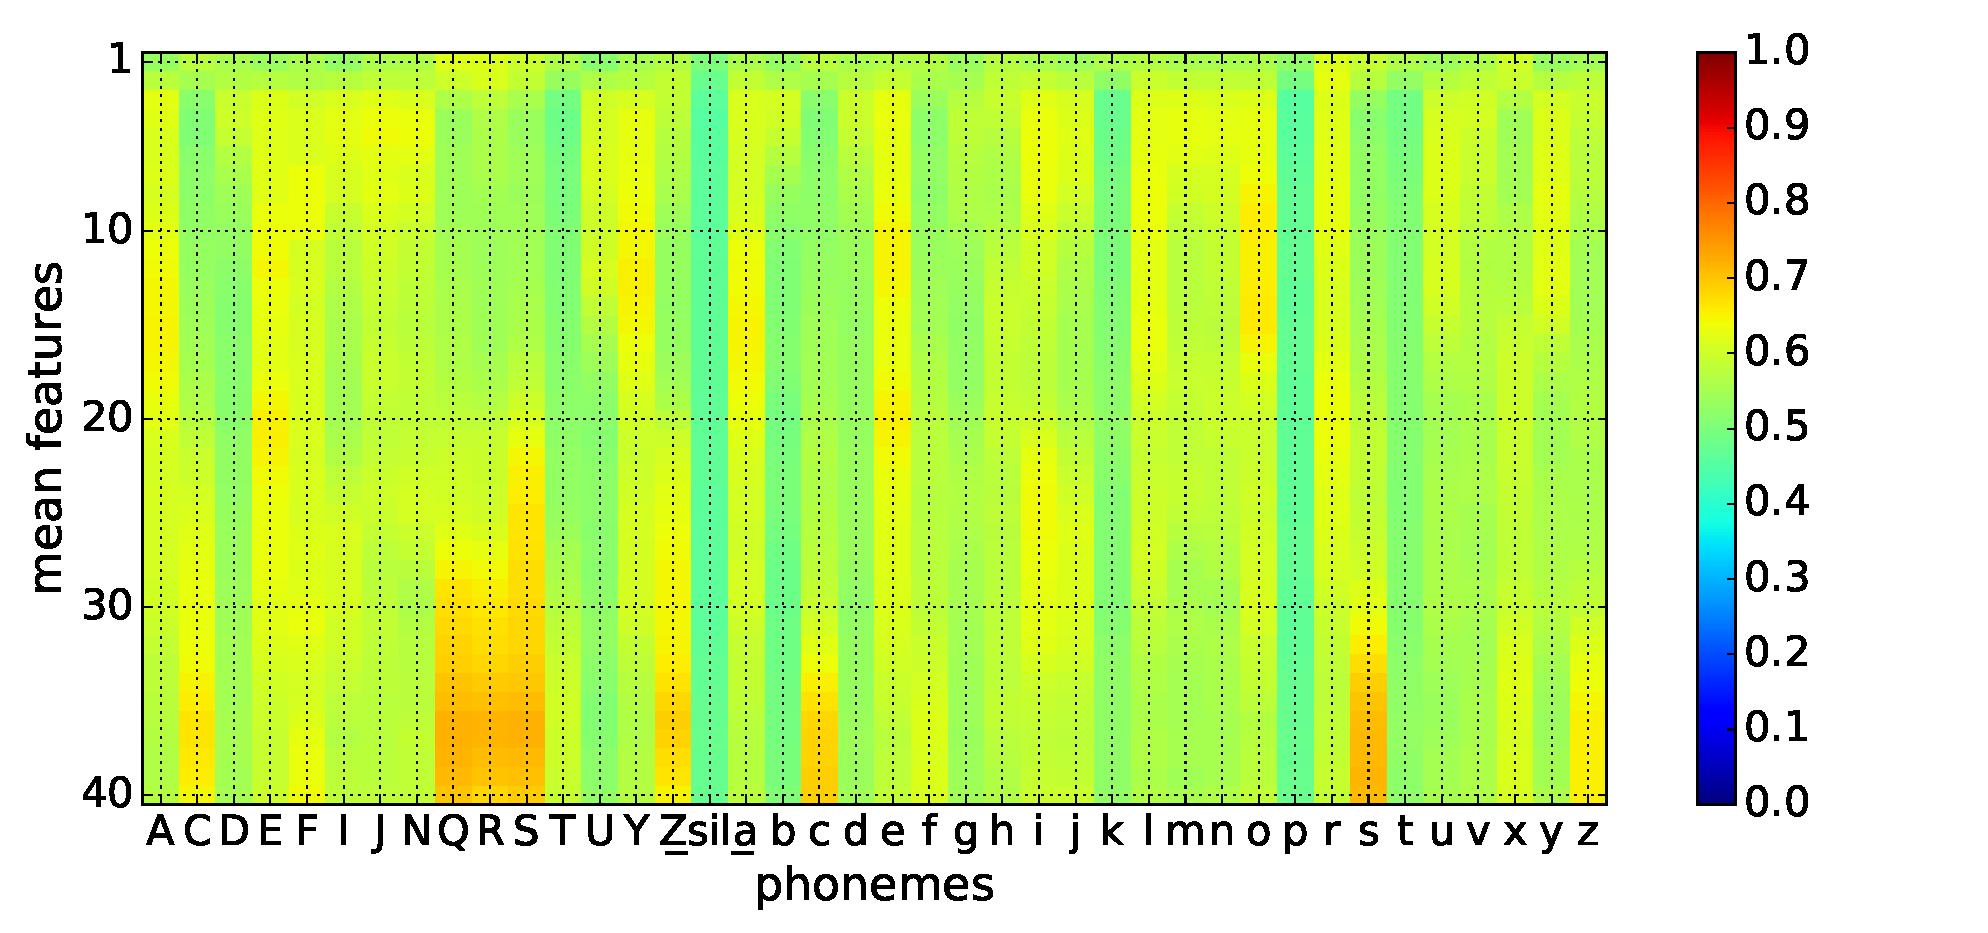
\includegraphics[width=\textwidth]{average_sample_10K_cs0_norm.eps}
\caption{Average sample for each phoneme, $ cs = 0 $.}
\label{fig:examples:speech_average_sample_cs0}
\end{figure}

For example, the pause (\texttt{"\_sil\_"}) is very similar to phoneme \texttt{"p"} having low values for all frequencies. Phonemes \texttt{"A"} and \texttt{"a"} also take a similar course, as well as high-frequency groups (\texttt{"Q"}, \texttt{"R"}, \texttt{"S"}) or (\texttt{"c"}, \texttt{"s"}, \texttt{"z"}).

Using the derived parameter settings ($ cs = 3 $) we end up with a feature vector of length $ 280 $. An example for each class is shown in \cref{fig:examples:speech_example_sample_cs3}. Average values can be found in \cref{app:supplementary_data}, \cref{fig:app:speech_average_sample_cs3}.

\begin{figure}[H]
\centering
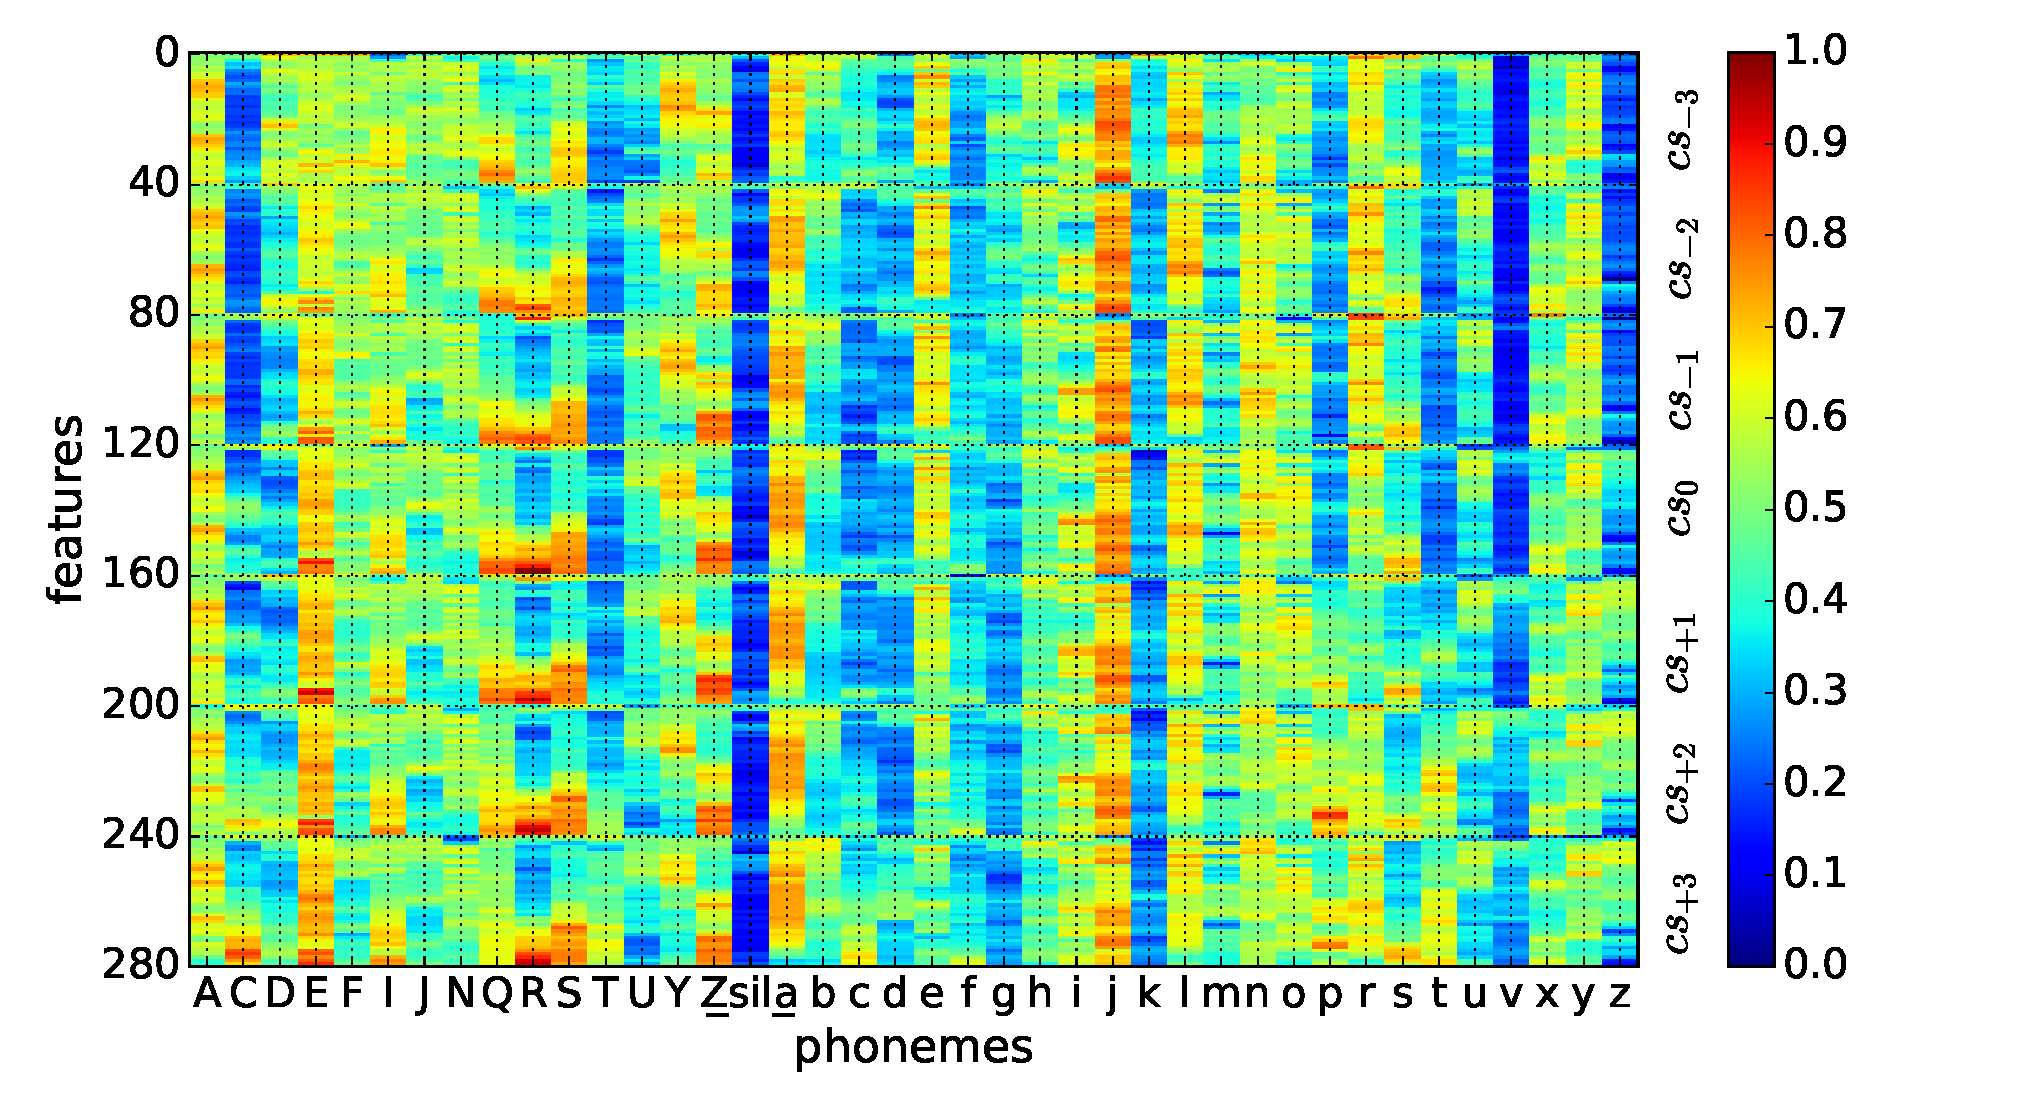
\includegraphics[width=\textwidth]{example_sample_10K_cs3_norm.eps}
\caption{Randomly selected sample for each phoneme, $ cs = 3 $.}
\label{fig:examples:speech_example_sample_cs3}
\end{figure}

\subsection*{Classification Results: Speech Dataset}
At first we must keep in mind that getting the best possible classification accuracy is not the goal in this work. Rather than spending months of computation time for training huge networks, we choose a simplier network structure and try to get the best out of it. Two different network structures were trained:

\begin{enumerate}
\item Network \texttt{[280, 50, 2, 50, 40]} (bottleneck\footnote{A bottleneck network contains a layer that consists of few nodes compared to the previous layers. It can be used to get a representation of the network input with reduced dimensionality.} network);
\item Network \texttt{[280, 100, 50, 40]}.
\end{enumerate}

The learning parameters for both networks are listed in \cref{tab:examples:speech_learning_parameters}.

\begin{table}[H]
\centering
\begin{tabular}{|l|c|l|c|}
\hline
\multicolumn{2}{|c|}{dataset} & \multicolumn{2}{c|}{learning parameters} \\ \hline
n samples / class    & 5000   & learning rate            & 0.07          \\ \hline
border size          & 3      & n epochs                 & 100           \\ \hline
context size         & 3      & batch size               & 10            \\ \hline
\end{tabular}
\caption{Phonemes: dataset and learning parameters.}
\label{tab:examples:speech_learning_parameters}
\end{table}

\subsubsection*{1. Network (bottleneck)}
The network with the bottleneck layer was trained to test accuracy $ 30\% $ ($ MSE' = 0.0105 $). A complete confusion matrix can be found in \cref{app:supplementary_data}, \cref{fig:app:speech_bottleneck_cm}. The confusion matrix helped us find phonemes that had been trained better compared to the others. We focused on phonemes with recall\footnote{Recall score is the ability of a classifier to find all the positive samples. It is defined as $ \frac{tp}{tp+fn} $, where $ tp $ is the number of true positives and $ fn $ the number of false negatives.} greater than $ 0.5 $.

The purpose of training a bottleneck network is the reduction of input's dimensionality. Using a layer with just two neurons usually does not lead to a high classification accuracy (also confirmed here), but the adventage is that it can be illustrated in 2D space.

For the selected phonemes, \cref{fig:examples:speech_bottleneck_result} shows the representation of testing samples in the bottleneck layer. We used the \textit{Sigmoid} transfer function, so all samples lie in $ [0,1] x [0,1] $.

\begin{figure}[H]
\centering
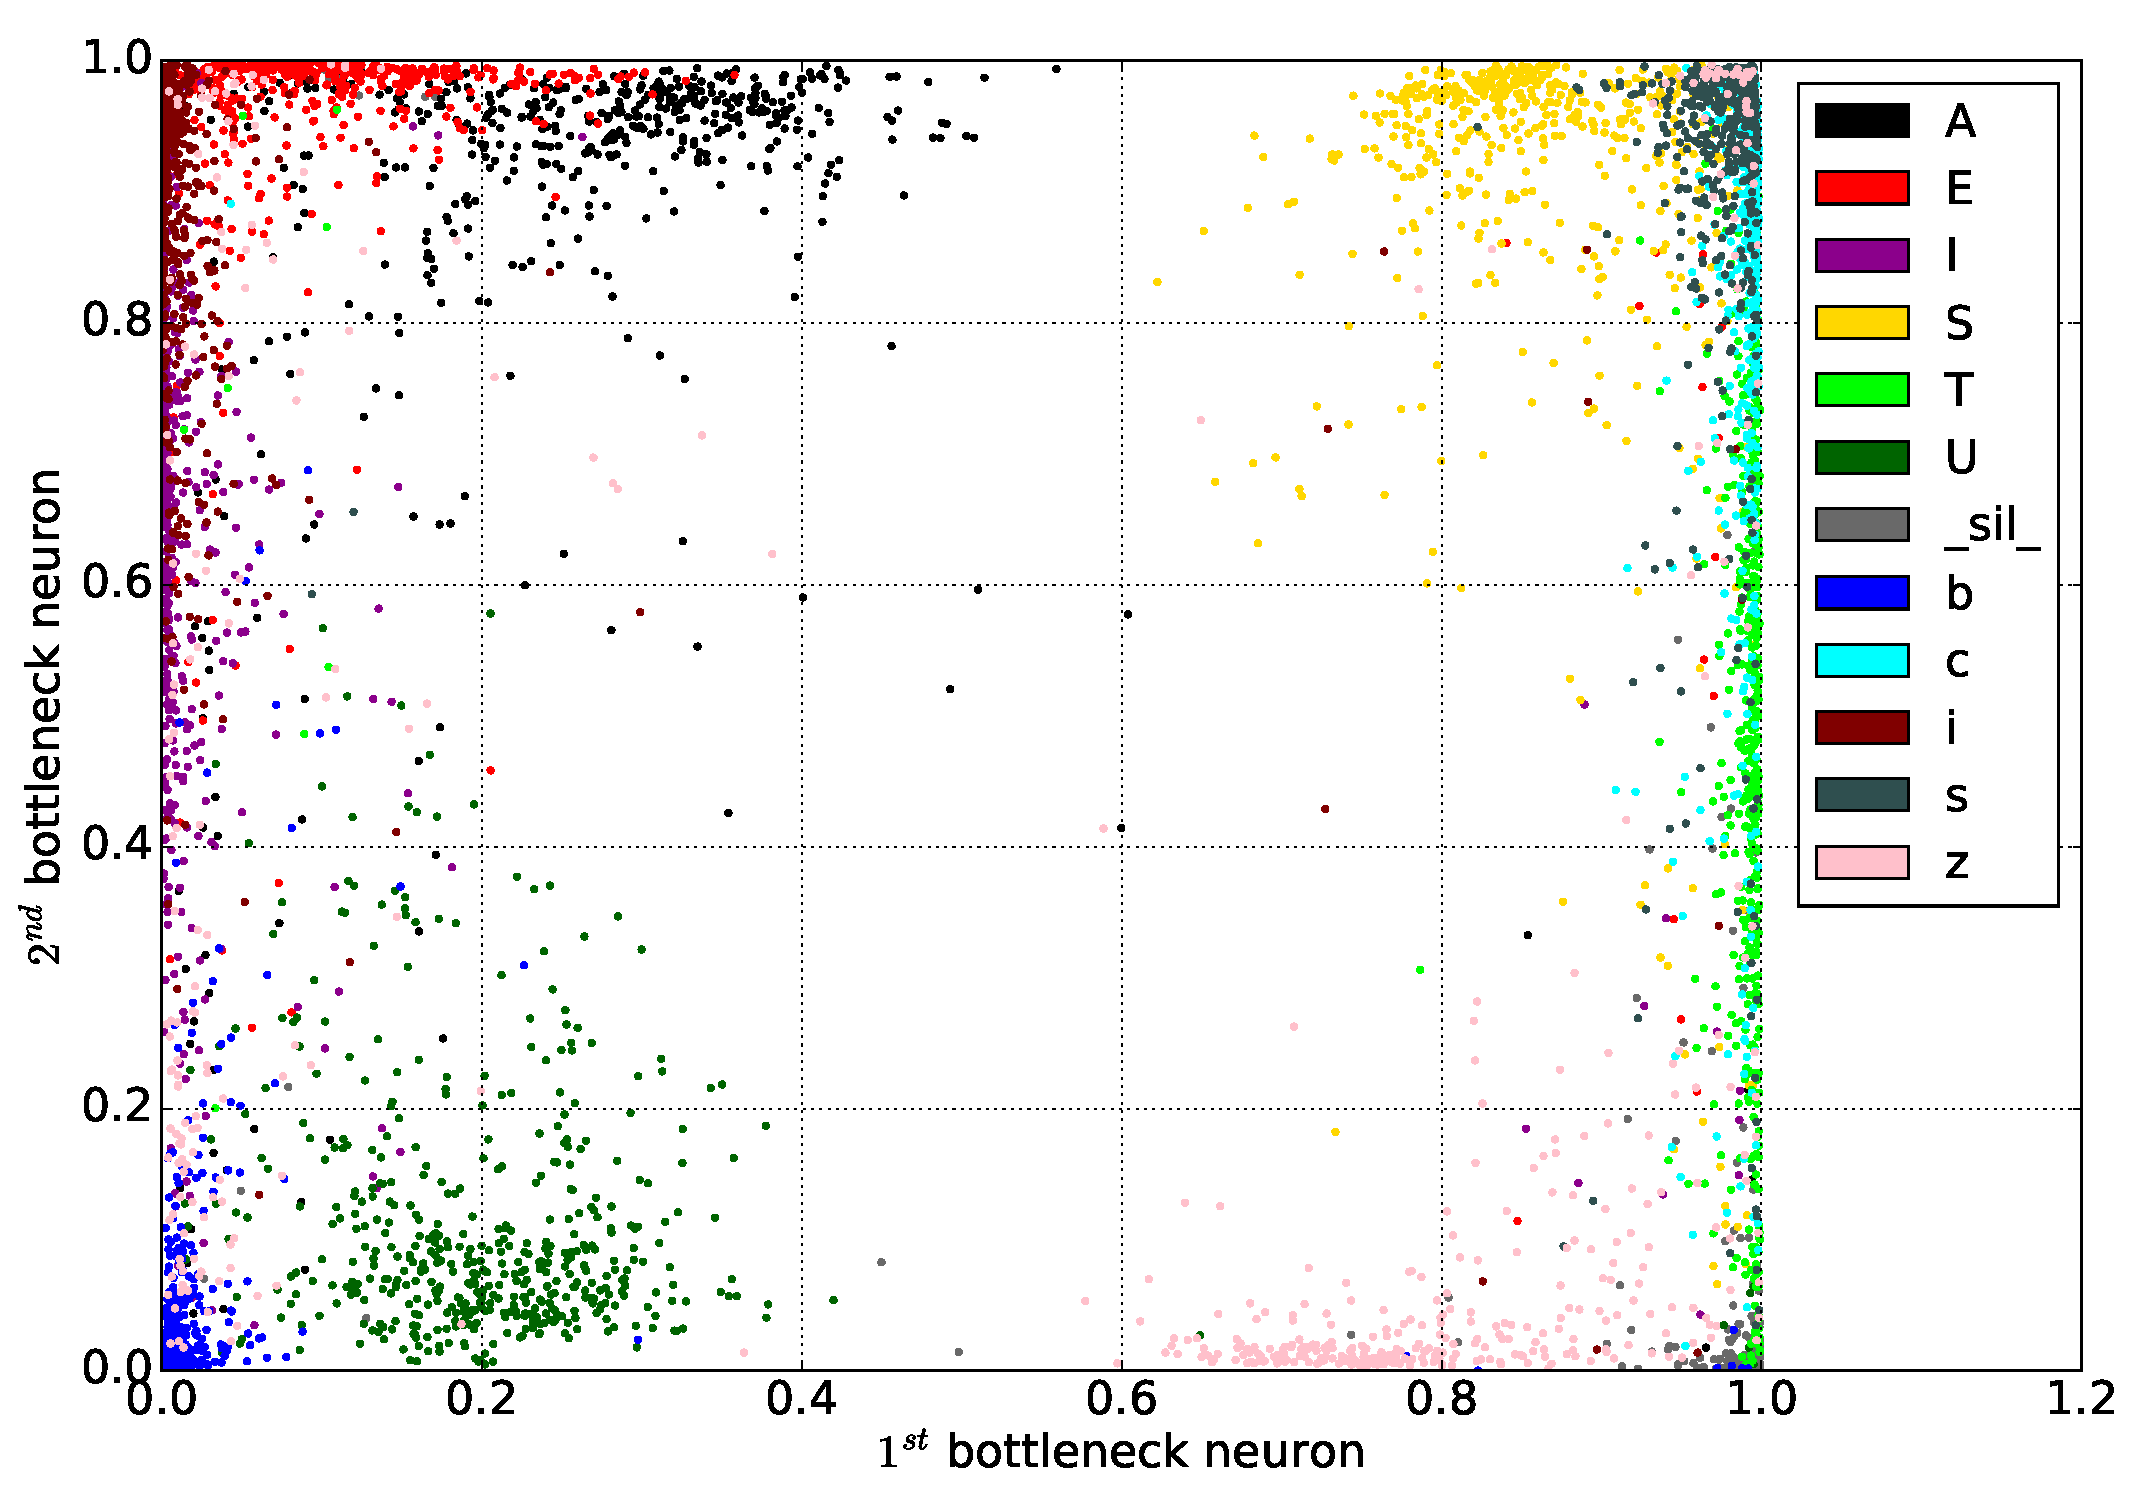
\includegraphics[width=\textwidth]{speech_bottleneck_result.eps}
\caption{Representation of individual phonemes in the 2D bottleneck layer (selected phonemes).}
\label{fig:examples:speech_bottleneck_result}
\end{figure}

The figure confirms some intuitive expectations. For example, samples of phoneme \texttt{"I"} are close to representations of phoneme \texttt{"i"} and also not far away from \texttt{"A"} and \texttt{"E"} samples. Another area contains samples of \texttt{"S"} together with \texttt{"s"} and \texttt{"c"} samples.

The bottleneck network with two neurons is a simple example of how the work in networks can be illustrated.

\subsubsection*{2. Network}
The second network with structure \texttt{[280, 100, 50, 40]} was trained with the same settings (\cref{tab:examples:speech_learning_parameters}). The learning ended with accuracy $ 63.8\% $ and $ MSE' = 0.0063 $. \cref{fig:examples:speech_net_cm} shows the complete confusion matrix.

\begin{figure}[H]
\centering
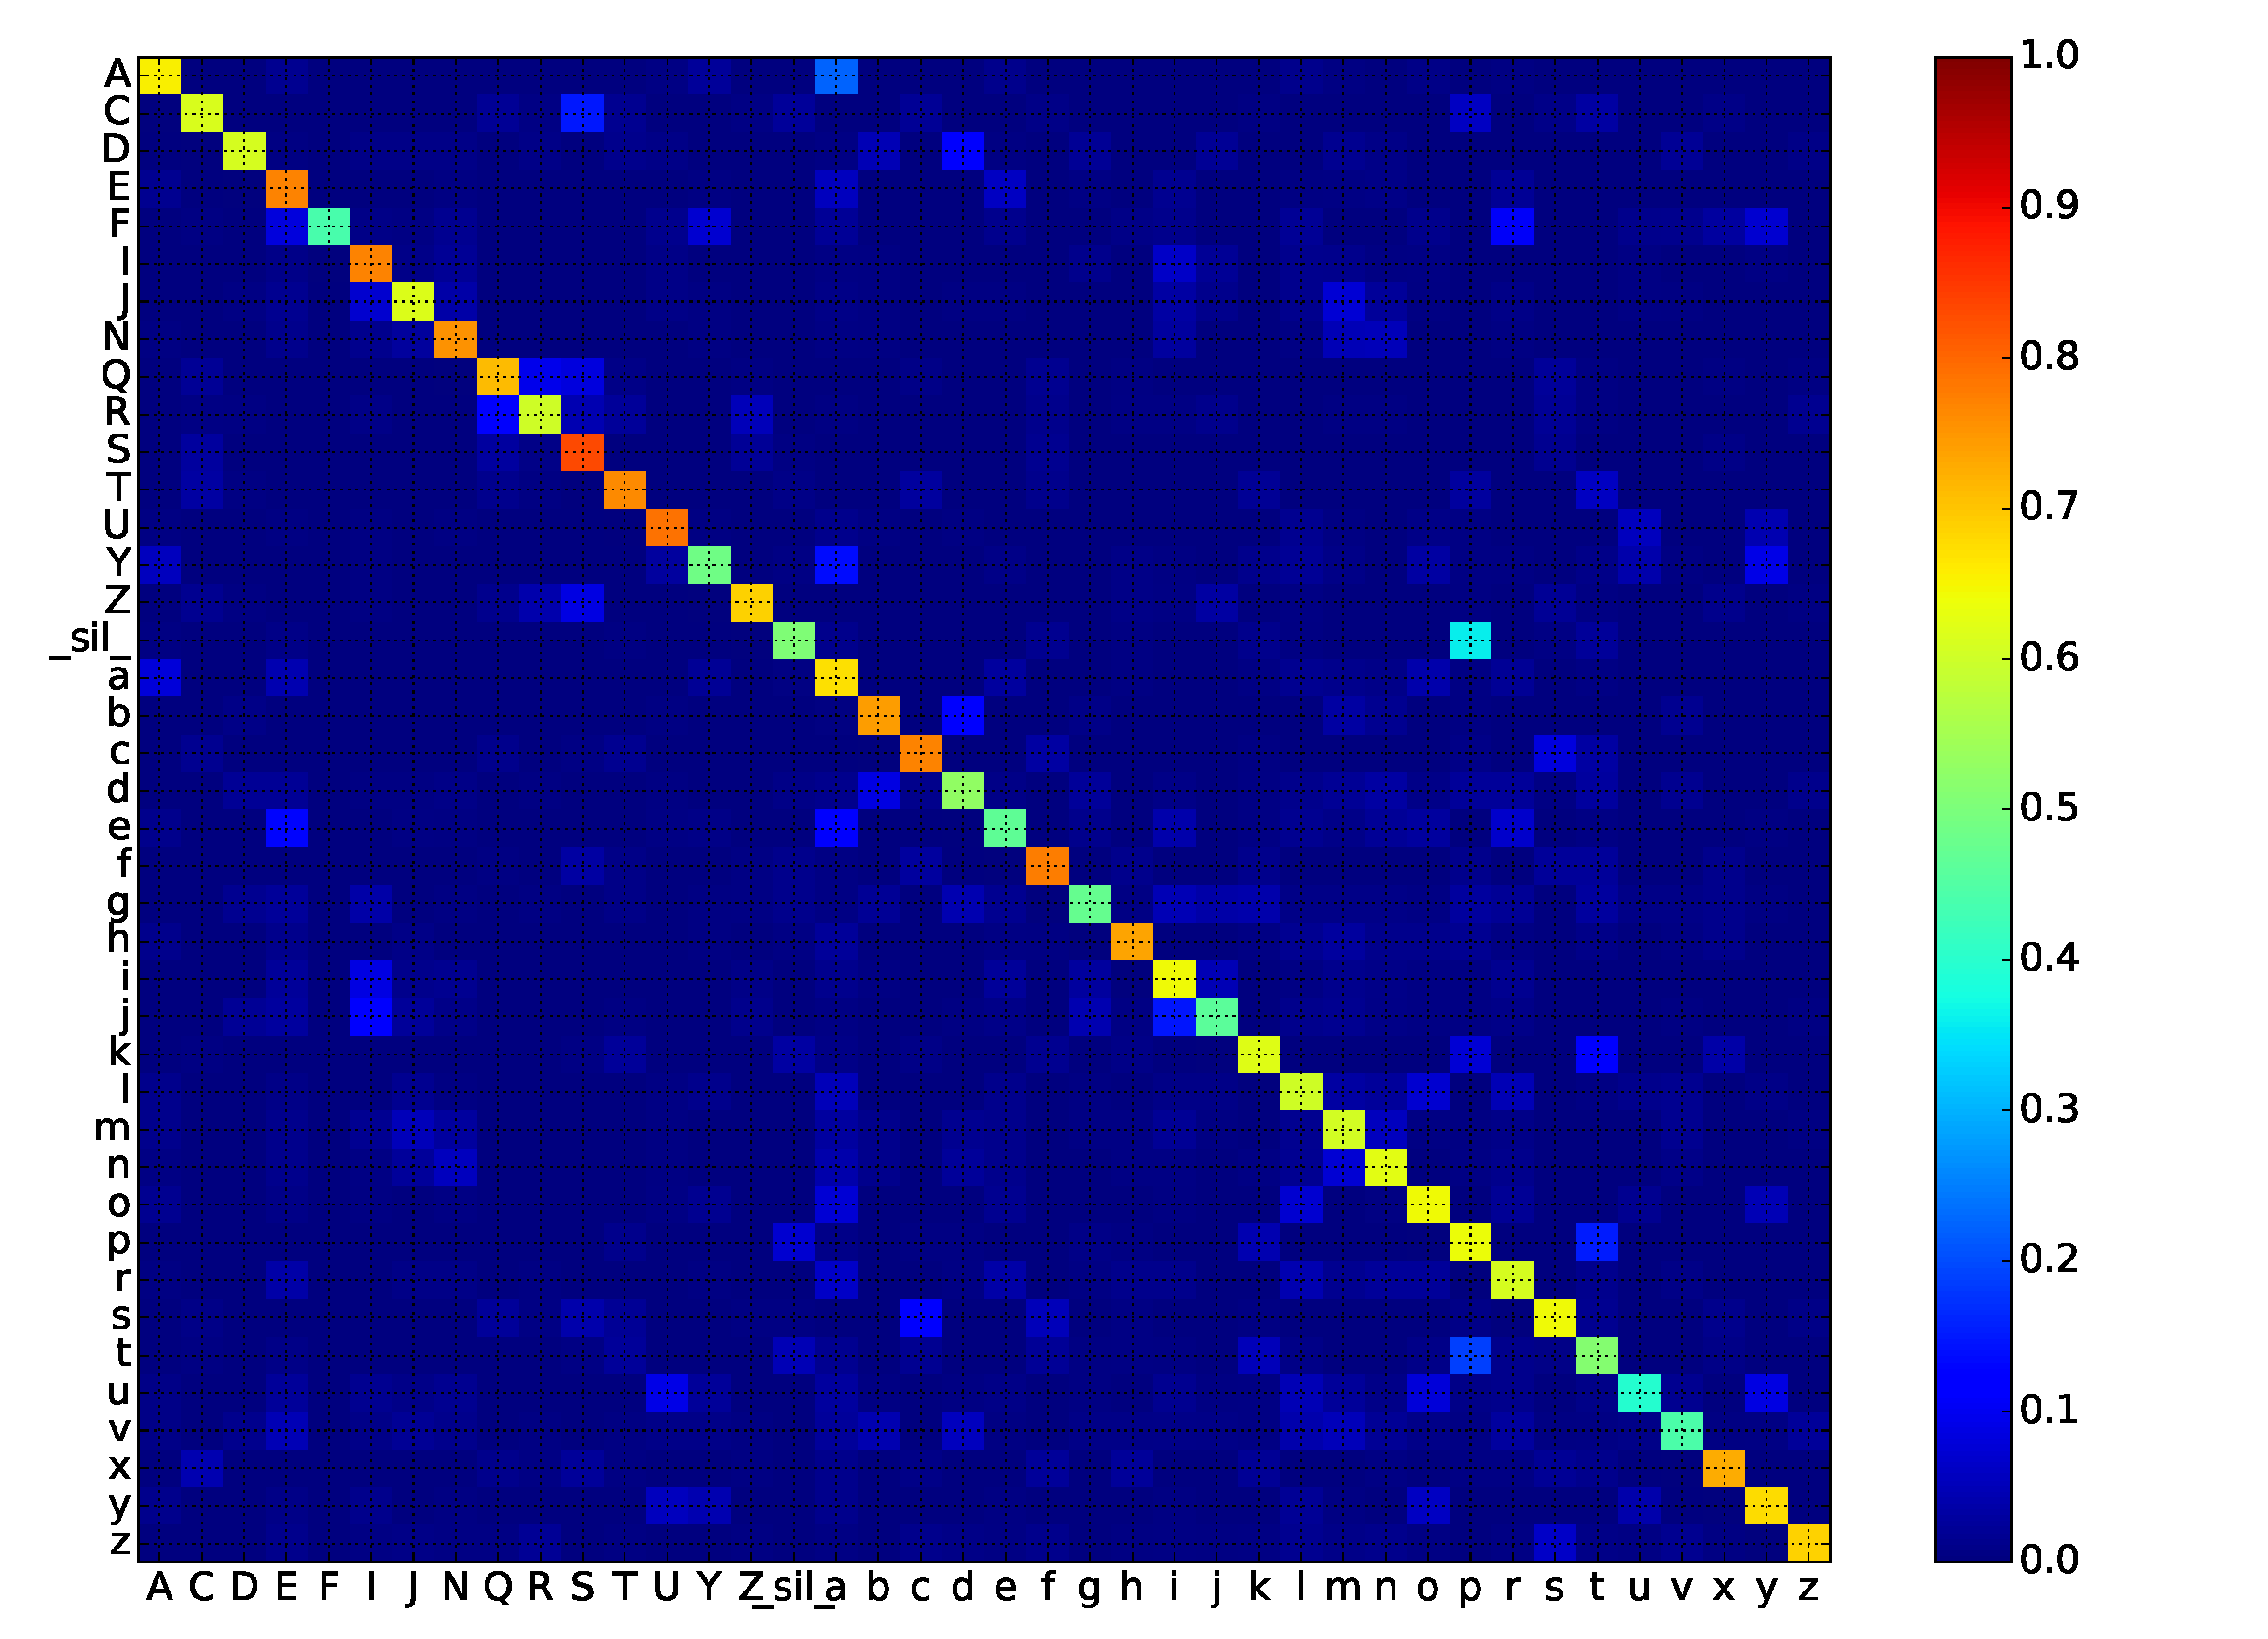
\includegraphics[width=\textwidth]{speech_net_cm.eps}
\caption{Confusion matrix of the classification results on the speech dataset.}
\label{fig:examples:speech_net_cm}
\end{figure}

\subsection*{Pruning Results: Speech Dataset}
The second network (\texttt{[280, 100, 50, 40]}) was pruned. In this case we sacrificed a few percent of classification accuracy and required $ req\_acc = 50\% $ only. The pruning process is tracked in \cref{fig:examples:speech_pruning_process}.

\begin{figure}[H]
\centering
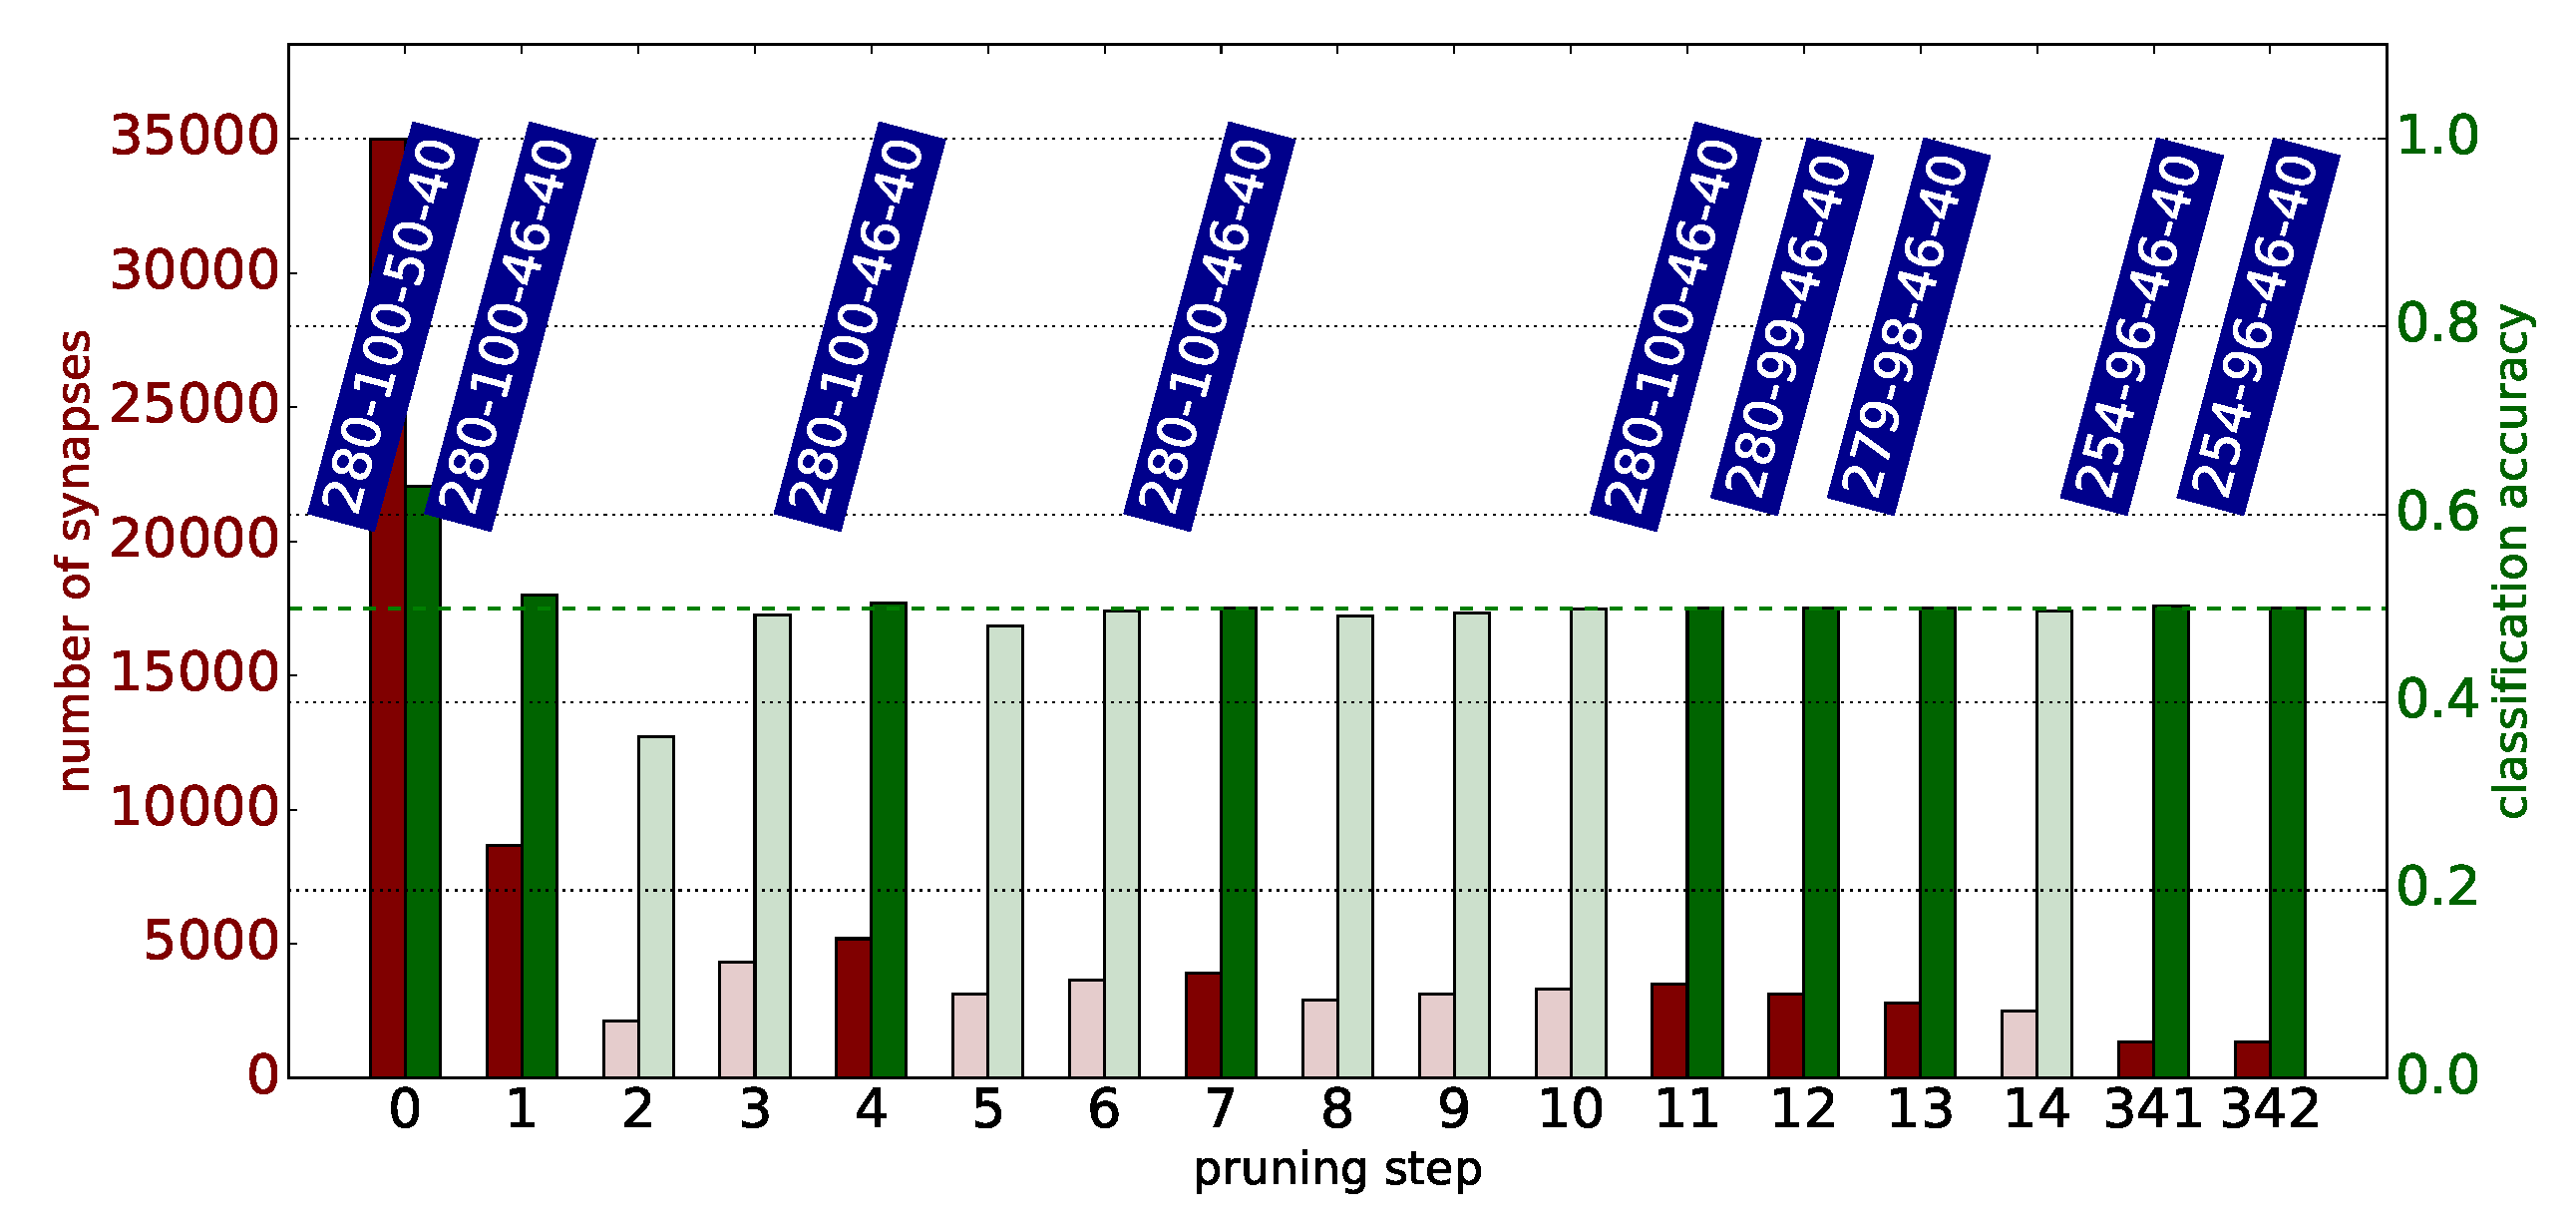
\includegraphics[width=\textwidth]{pruning_process_speech.eps}
\caption{Illustration of the pruning procedure applied on SPEECH dataset (selected observation). Required accuracy: $ 50\% $.}
\label{fig:examples:speech_pruning_process}
\end{figure}

The initial number of synapses $ 35000 $ was reduced to $ 1344 $. Eight hidden neurons (four in each hidden layer) were cut out. Regarding the input layer $ 26 $ neurons were cut out, which reveals that only $ 254 $ out of $ 280 $ features are neccessarry to obtain the classification accuracy of $ 50\% $ on validation data.

The dimensionality reduction is not that significant for this example compared to the others (e.g. MNIST). Also we require a low classification accuracy. However, one must remember that we work with a $ 40 $-class problem, which is far from trivial. In the following section we try to find some patterns in the results, which could demystify what is going on in the network.

\subsection*{Feature Selection and Pathing: Speech Dataset}